\documentclass[referee,lineno,pdflatex,sn-mathphys-num]{sn-jnl}

% ============================================================================
% PACKAGES
% ============================================================================
\usepackage[utf8]{inputenc}
\usepackage[T1]{fontenc}
\usepackage{microtype}

% Graphics
\usepackage{graphicx}
\graphicspath{{figures/}}
\usepackage{tikz}
\usetikzlibrary{arrows.meta,positioning,fit}

% Mathematics
\usepackage{amsmath}
\usepackage{amssymb}
\usepackage{amsfonts}
\usepackage{amsthm}
\usepackage{mathtools}
\usepackage{bm}

% Theorem environments
\theoremstyle{thmstylethree}
\newtheorem{definition}{Definition}[section]
\newtheorem{assumption}{Assumption}[section]
\newtheorem{example}{Example}[section]

\theoremstyle{thmstyletwo}
\newtheorem{remark}{Remark}[section]

\theoremstyle{thmstyleone}
\newtheorem{theorem}{Theorem}[section]
\newtheorem{proposition}{Proposition}[section]
\newtheorem{lemma}{Lemma}[section]
\newtheorem{corollary}{Corollary}[section]

% Tables
\usepackage{booktabs}
\usepackage{array}
\usepackage{multirow}
\usepackage{siunitx}
\usepackage{enumitem}
\usepackage{threeparttable}
\usepackage{setspace}

% Colors
\usepackage{xcolor}
\definecolor{darkblue}{RGB}{0,51,102}
\definecolor{darkred}{RGB}{153,0,0}
\definecolor{darkgreen}{RGB}{0,102,51}

\hypersetup{
    colorlinks=true,
    linkcolor=darkblue,
    citecolor=darkblue,
    urlcolor=darkblue,
    unicode=true,
    pdftitle={Boundary Information Geometry for S-box Side-Channel Leakage},
}

% Custom commands
\newcommand{\F}{\mathbb{F}}
\newcommand{\R}{\mathbb{R}}
\newcommand{\E}{\mathbb{E}}
\newcommand{\KL}{D_{\mathrm{KL}}}
\newcommand{\FIM}{\mathcal{I}}
\newcommand{\HW}{\mathrm{HW}}
\newcommand{\NL}{\mathrm{NL}}
\newcommand{\DU}{\delta}
\newcommand{\DDT}{\mathrm{DDT}}
\newcommand{\LAT}{\mathrm{LAT}}
\newcommand{\WHT}{\widehat}
\newcommand{\tr}{\mathrm{tr}}
\newcommand{\vol}{\mathrm{vol}}
\DeclareMathOperator{\Esym}{\mathbb{E}}
\DeclareMathOperator{\Cov}{\mathrm{Cov}}
\DeclareMathOperator{\Var}{\mathrm{Var}}
\DeclareMathOperator*{\argmin}{arg\,min}
\DeclareMathOperator*{\argmax}{arg\,max}
\newcommand{\inner}[2]{\langle #1,\, #2 \rangle}

% Shorthand for {0,1}^n
\newcommand{\Bn}{\{0,1\}^s}
\newcommand{\B}[1]{\{0,1\}^{#1}}
\newcommand{\Z}{\mathbb{Z}}

\title[Boundary Information Geometry for S-box Side-Channel Leakage]{
Boundary Information Geometry for S-box Side-Channel Leakage:
Walsh Covariance, Active Fisher Structure, and CPA Belief Dynamics}

\abstract{
Side-channel attacks on lightweight block ciphers often reduce locally to
distinguishing key hypotheses through leakage generated by bijective S-boxes.
This paper develops an information-geometric model for these finite
key-induced distributions while separating three security-relevant spaces: the
singular distributions induced by exact key hypotheses, the regular
full-support exponential family used for Fisher geometry, and the adversary's
posterior belief simplex.  For an $s$-bit bijective S-box $S$ and key
hypothesis $k$, the exact distribution
$P_k(a,b)=2^{-s}\mathbf 1[b=S(a\oplus k)]$ is supported on one graph inside
$\{0,1\}^{2s}$ and therefore lies on the boundary of the probability simplex.
Walsh characters give the key-translation rule
$\widehat P_k(\alpha,\beta)=(-1)^{\alpha\cdot k}\widehat P_0(\alpha,\beta)$.
Using this rule as a structural input, we derive closed-form boundary
covariance matrices and prove that, for every bijective S-box, their active
subspace has dimension $2^s-1$ and active eigenvalues equal $2^s$ in the
unnormalised Walsh basis.  We then interpret correlation power analysis under
Gaussian leakage as Bayesian dynamics on the key-belief simplex.  The
Hamming-weight variance $s/(4\sigma^2)$ is a bijectivity-driven baseline,
whereas pairwise likelihood gaps determine key-hypothesis discrimination and
worst-case posterior-odds growth.  Reproducible computations and Monte Carlo
CPA simulations for PRESENT, GIFT, and SKINNY show how S-boxes with the same
Walsh-amplitude distribution can have distinct hard and easy key differences
under Hamming-weight leakage while sharing the boundary covariance invariants
forced by bijectivity.
}

\keywords{cybersecurity, side-channel analysis, correlation power analysis,
S-box, information geometry, Fisher--Rao metric, Walsh--Hadamard transform,
Bayesian inference}

\begin{document}
\maketitle
\doublespacing

%\tableofcontents
%\newpage

% ============================================================================
% ============================================================================
% Begin inlined file: sections/introduction.tex
% ============================================================================
% ============================================================================
% SECTION 1: INTRODUCTION
% ============================================================================
\section{Introduction}\label{sec:intro}

\subsection{Motivation}

Side-channel attacks use implementation leakage in addition to the abstract
cipher description.  In many attacks on lightweight block ciphers, the
local statistical object is a keyed S-box computation: an adversary observes or
controls an input nibble or byte, measures a noisy leakage trace, and compares
key hypotheses through predicted intermediate values.  Correlation power
analysis (CPA) is the standard example: each trace updates the adversary's
belief about the key using a leakage model such as Hamming weight.

The exact distribution induced by a keyed bijective S-box is not a smooth
interior point of a probability simplex.  For an $s$-bit bijective S-box
$S:\{0,1\}^s\to\{0,1\}^s$ and key hypothesis $k\in\{0,1\}^s$, the pair
$(a,b)$ with uniform $a$ and $b=S(a\oplus k)$ is supported on only $2^s$ points
of the $2^{2s}$-point input-output space.  Hence $P_k$ is a singular boundary
distribution.  This matters because ordinary Fisher--Rao tensors, geodesics,
and dual-flat coordinates are defined on full-support statistical models, not
directly at support-deficient endpoints.

This paper develops a boundary information-geometric framework for this
side-channel setting.  The central discipline is to keep separate three
objects that are often conflated in informal geometric descriptions:
\begin{enumerate}[label=\normalfont(\roman*)]
  \item the regular full-support Walsh exponential family, where ordinary
  Fisher geometry is valid;
  \item the finite boundary orbit of exact key-induced S-box distributions;
  \item the adversary's posterior belief simplex over key hypotheses, where
  CPA updates take place.
\end{enumerate}
This separation makes it possible to use information geometry in a controlled
way: boundary distributions are represented through covariance limits, whereas
Bayesian key recovery remains a regular trajectory on the belief simplex as
long as the prior has full support and the leakage likelihood is positive.

For cybersecurity and hardware-security evaluation, the practical output of
this separation is a
diagnostic workflow for identifying which quantities are unavoidable
consequences of bijectivity, which quantities are artefacts of the chosen
Walsh coordinates, and which quantities actually affect CPA discrimination.
In particular, for Hamming-weight leakage the scalar variance is identical for
all bijective S-boxes of the same width, but the pairwise gaps between key
hypotheses need not be identical.  Those gaps determine the expected
posterior-odds growth against wrong keys and therefore identify the key
differences that are locally hardest or easiest for a CPA adversary to reject.

\begin{figure}[t]
\centering
\resizebox{\textwidth}{!}{%
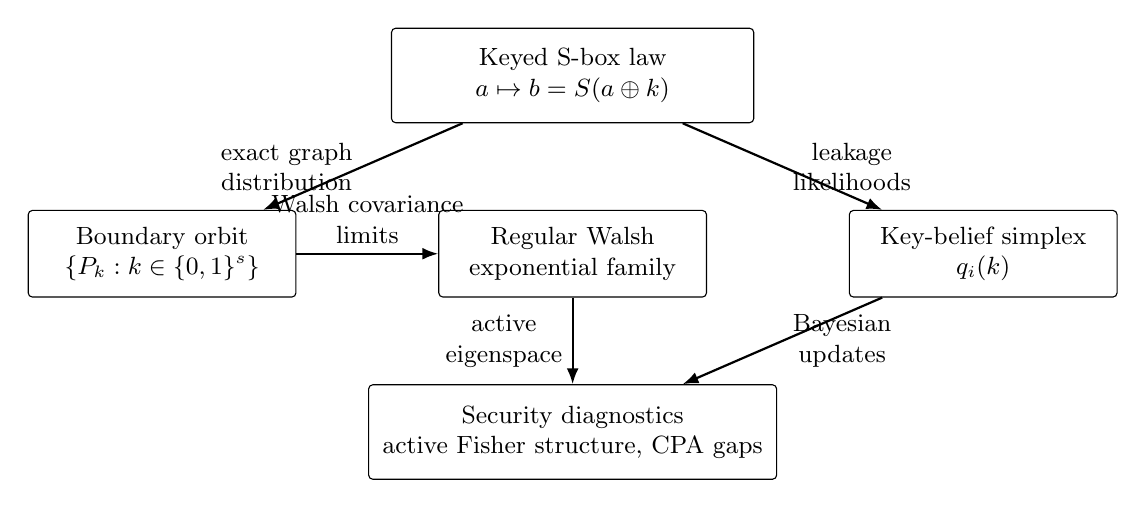
\begin{tikzpicture}[
  font=\small,
  node distance=11mm and 12mm,
  box/.style={
    draw,
    rounded corners=1.5pt,
    align=center,
    inner sep=5pt,
    minimum width=34mm,
    minimum height=11mm
  },
  wide/.style={
    draw,
    rounded corners=1.5pt,
    align=center,
    inner sep=5pt,
    minimum width=46mm,
    minimum height=12mm
  },
  arr/.style={-{Latex[length=2mm]},thick}
]
\node[wide] (sbox) {Keyed S-box law\\$a\mapsto b=S(a\oplus k)$};
\node[box, below left=of sbox] (boundary) {Boundary orbit\\$\{P_k:k\in\{0,1\}^s\}$};
\node[box, below=of sbox] (interior) {Regular Walsh\\exponential family};
\node[box, below right=of sbox] (belief) {Key-belief simplex\\$q_i(k)$};
\node[wide, below=of interior] (diagnostics) {Security diagnostics\\active Fisher structure, CPA gaps};

\draw[arr] (sbox) -- node[left,align=center] {exact graph\\distribution} (boundary);
\draw[arr] (sbox) -- node[right,align=center] {leakage\\likelihoods} (belief);
\draw[arr] (boundary) -- node[above,align=center] {Walsh covariance\\limits} (interior);
\draw[arr] (interior) -- node[left,align=center] {active\\eigenspace} (diagnostics);
\draw[arr] (belief) -- node[right,align=center] {Bayesian\\updates} (diagnostics);
\end{tikzpicture}
}
\caption{Boundary-to-belief framework. The exact keyed S-box laws lie on a
singular boundary orbit, the Fisher calculations are made in a regular Walsh
exponential family or in boundary covariance limits, and CPA updates evolve on
the separate key-belief simplex.}
\label{fig:framework}
\end{figure}

\subsection{Relation to prior work}

The information-geometric background is the Fisher--Rao and dual-affine
geometry of finite statistical models and regular exponential families
\cite{amari2000methods,ay2017information,chentsov1982statistical}.  The
closest coding-theoretic precedent is the work of Ikeda, Tanaka, and Amari on
LDPC and turbo codes~\cite{ikeda2004information}: parity-check statistics
define a regular information-geometric model and decoding trajectories are
interpreted through projections.  Here, the sufficient statistics are
Walsh--Hadamard characters on S-box input-output pairs, and the inference
trajectory is the CPA posterior over key hypotheses.

On the cryptographic side, the work is related to classical Walsh/LAT and DDT
analysis of vectorial Boolean functions and S-boxes, including Nyberg's
differential uniformity~\cite{nyberg1994differentially}.  Four-bit S-boxes and
optimal 4-bit permutations have been classified in the Boolean-function
literature, notably by Leander and Poschmann~\cite{leander2007classification}.
Recent geometric viewpoints in symmetric cryptanalysis also include geometric
formulations of linear and differential cryptanalysis
\cite{beyne2021geometric,beyne2022quasidifferential}.
The present paper builds on this background by asking which
information-geometric objects are associated with exact keyed S-box
distributions and how those objects connect to side-channel belief updates.
This positioning uses existing 4-bit S-box classifications as prior
cryptographic knowledge and focuses on the local leakage distributions used in
CPA.

On the side-channel side, the leakage model and posterior update are consistent
with differential and correlation power analysis
\cite{kocher1999differential,brier2004correlation} and with
information-theoretic analyses of key recovery attacks
\cite{standaert2009unified,veyrat2009adaptive}.  The present framework gives a
formal model for separating baseline invariants forced by bijectivity from
pairwise leakage gaps that control key-hypothesis discrimination.

Table~\ref{tab:sota-positioning} summarizes the intended position of the
framework relative to standard S-box and side-channel criteria.

\begin{table}[t]
\centering
\caption{Relation to existing metrics.}
\label{tab:sota-positioning}
\footnotesize
\setlength{\tabcolsep}{3pt}
\begin{tabular}{@{}p{0.22\textwidth}p{0.34\textwidth}p{0.34\textwidth}@{}}
\toprule
Metric or framework & Standard role & Role in this paper \\
\midrule
Walsh/LAT spectrum & Measures linear correlations of vectorial Boolean
functions and supports nonlinearity analysis. & Provides coordinates for the
key-induced boundary orbit and for closed-form covariance diagnostics. \\
DDT and differential uniformity & Measures differential propagation and
classical S-box resistance to differential attacks~\cite{nyberg1994differentially}. &
Used as part of the surrounding S-box context for separating classical
cryptographic criteria from leakage-geometry diagnostics. \\
4-bit S-box classification & Classifies small permutations up to established
equivalences~\cite{leander2007classification}. & Used as prior cryptographic
knowledge for interpreting the local leakage geometry. \\
CPA and DPA likelihood models & Explain key recovery from noisy implementation
leakage~\cite{kocher1999differential,brier2004correlation}. & Interpreted as
Bayesian dynamics on the key-belief simplex with pairwise likelihood gaps. \\
Mutual information and key-rank measures & Quantify leakage and attack success
at the experiment or trace-distribution level~\cite{standaert2009unified,veyrat2009adaptive}. &
Complemented by local structural diagnostics for keyed S-box laws and
posterior-odds growth. \\
Information geometry of codes & Studies decoding and projections in regular
statistical models~\cite{ikeda2004information}. & Adapted to singular S-box
graph distributions by separating boundary covariance, regular interiors, and
belief-simplex updates. \\
\bottomrule
\end{tabular}
\end{table}

\subsection{Setting and notation}

Throughout, $s\geq1$ denotes the S-box width in bits,
$S:\B{s}\to\B{s}$ is a fixed bijection, $k\in\B{s}$ is a key hypothesis, and
$a\in\B{s}$ is a uniformly distributed plaintext nibble or byte.  All additions
inside bit strings are over $\F_2$.  The inner product is
$\alpha\cdot a=\bigoplus_{i=1}^s \alpha_i a_i$.  For
$(\alpha,\beta)\in\B{s}\times\B{s}$, the Walsh character is
\[
  \chi_{\alpha\beta}(a,b)=(-1)^{\alpha\cdot a\oplus\beta\cdot b}.
\]
We write $N=2^s$ and $\mathcal X=\B{s}\times\B{s}$.

\subsection{Contributions}\label{subsec:contributions}

\begin{enumerate}[label=\textbf{C\arabic*.}]

\item \textbf{Boundary model for key-induced S-box distributions.}
We model the exact keyed S-box law
\[
  P_k(a,b)=2^{-s}\mathbf 1[b=S(a\oplus k)]
\]
as a boundary distribution on the input-output simplex.  The Walsh translation
rule
\[
  \widehat P_k(\alpha,\beta)
  =(-1)^{\alpha\cdot k}\widehat P_0(\alpha,\beta)
\]
is used as a coordinate identity for the finite key orbit and as the algebraic
input for the covariance and leakage diagnostics.

\item \textbf{Closed-form boundary covariance and active Fisher structure.}
We derive the boundary covariance form
\[
  \mathcal I^{\partial}_{ij}(k)=\operatorname{Cov}_{P_k}(T_i,T_j)
\]
in Walsh coordinates and prove that, for every bijection $S:\B{s}\to\B{s}$,
this matrix has rank $2^s-1$ and active eigenvalues all equal to $2^s$ in the
unnormalised Walsh basis.  Thus the active boundary geometry is a structural
property of bijective S-box graphs shared by the three illustrative 4-bit
examples.

\item \textbf{Regular interior and belief-simplex geometry.}
We explicitly separate the regular Walsh exponential family, where the usual
Amari dual-flat structure and Pythagorean identities apply, from the singular
boundary orbit.  The adversary's key belief is treated as a separate full-
support simplex, equipped with its own Fisher--Rao metric.

\item \textbf{CPA as Bayesian belief dynamics with pairwise leakage gaps.}
Under Gaussian leakage, each CPA trace is represented as a Bayesian update on
the key-belief simplex.  The Hamming-weight variance
$s/(4\sigma^2)$ is identified as a baseline forced by bijectivity and uniform
inputs.  The quantities that distinguish key hypotheses are the pairwise
separations
\[
  \Delta(k,k^*)=\frac1{2^s}\sum_a
  \bigl(f(S(a\oplus k^*))-f(S(a\oplus k))\bigr)^2,
\]
which determine expected log-Bayes gains.

\item \textbf{Reproducible diagnostics on lightweight S-boxes.}
For PRESENT, GIFT, and SKINNY, we compute Walsh spectra, boundary covariance
matrices, local spectral separation proxies, pairwise Hamming-weight leakage
gaps, Monte Carlo CPA success curves, and the projected active-eigenspace
curvature diagnostic.  The examples
are used to separate invariants forced by bijectivity or by the shared Walsh
amplitude distribution from quantities that can vary across S-boxes.  The
pairwise-gap tables and CPA simulations identify the hard key differences and
trace-dependent key-rank behavior under the assumed leakage model.
\end{enumerate}

\subsection{Model coverage}\label{subsec:scope}

The paper focuses on isolated bijective S-boxes under uniform inputs and on an
additive Gaussian leakage model for CPA belief updates.  This coverage matches
the local leakage setting in which S-box output predictions drive non-profiled
CPA.  Extensions to complete multi-round ciphers, masking, higher-order
leakage, non-Gaussian leakage, profiled attacks, and implementation-specific
trace effects can be built by adding the corresponding leakage and cipher
propagation models to the boundary-distribution and belief-update framework.

% ============================================================================
% End inlined file: sections/introduction.tex
% ============================================================================
% ============================================================================
% Begin inlined file: sections/background.tex
% ============================================================================
% ============================================================================
% SECTION 2: BACKGROUND
% ============================================================================
\section{Background}\label{sec:background}

\subsection{S-boxes and the Walsh--Hadamard transform}

An \emph{$s$-bit S-box} is a bijection $S : \B{s} \to \B{s}$.
The $i$-th output bit is a Boolean function $S_i : \B{s}\to\{0,1\}$.

\begin{definition}[Walsh--Hadamard Transform]\label{def:wht}
The Walsh--Hadamard transform (WHT) of $S$ at $(\alpha,\beta)\in\B{s}\times\B{s}$ is:
\begin{equation}\label{eq:wht}
  \WHT{S}(\alpha,\beta)
  = \sum_{a\in\B{s}} (-1)^{\alpha\cdot a\,\oplus\,\beta\cdot S(a)}
  \;\in\; \{-2^s,\ldots,+2^s\},
  \qquad 2\mid\WHT{S}(\alpha,\beta).
\end{equation}
By convention $\WHT{S}(0,0)=2^s$.
\end{definition}

The WHT encodes the two fundamental cryptographic properties of $S$:
\begin{itemize}
  \item \textbf{Nonlinearity}:
    $\NL(S) = 2^{s-1} - \tfrac{1}{2}\max_{(\alpha,\beta)\neq(0,0)}|\WHT{S}(\alpha,\beta)|$.
  \item \textbf{Differential uniformity}:
    $\DU(S) = \max_{\Delta_{\mathrm{in}}\neq 0,\,\Delta_{\mathrm{out}}}
    \bigl|\{a : S(a)\oplus S(a\oplus\Delta_{\mathrm{in}})=\Delta_{\mathrm{out}}\}\bigr|$.
\end{itemize}

The \emph{Linear Approximation Table} (LAT) entry is $\LAT_S(\alpha,\beta) = \WHT{S}(\alpha,\beta)/2$.
For any S-box, Parseval's identity gives:
\begin{equation}\label{eq:parseval}
  \sum_{(\alpha,\beta)\in\B{s}\times\B{s}} \WHT{S}(\alpha,\beta)^2 = 2^{2s}\cdot 2^s = 2^{3s}.
\end{equation}

\begin{example}[PRESENT S-box]\label{ex:present}
The PRESENT-80 S-box ($s=4$) is the hexadecimal table
$S = \texttt{[C,5,6,B,9,0,A,D,3,E,F,8,4,7,1,2]}$.
Its nonlinearity is $\NL(S)=4$ and differential uniformity $\DU(S)=4$.
\end{example}

\subsubsection{Remark on 4-bit S-box classification}

The 4-bit case is small enough that strong classification results are
available.  In particular, optimal 4-bit S-boxes have been studied up to the
standard equivalence relations used for vectorial Boolean functions
\cite{leander2007classification}.  The numerical examples in
Section~\ref{sec:numerical} use this classification background to provide
reproducible side-channel diagnostics for widely used lightweight S-boxes and
illustrate which information-geometric quantities are forced by bijectivity or
by common Walsh spectra.

\subsection{Information geometry: essentials}\label{subsec:ig}

We collect the minimal background from
Amari and Nagaoka~\cite{amari2000methods}
and Ay et al.~\cite{ay2017information} required in the sequel.

\subsubsection{Statistical manifolds and the Fisher metric}

Let $\mathcal{X}$ be a finite set with $|\mathcal{X}|=N$.
The \emph{probability simplex} is
$\Delta_{N-1} = \{p\in\R^N : p_x\geq 0,\; \sum_x p_x = 1\}$.
Its interior $\mathring{\Delta}_{N-1}$ is an $(N-1)$-dimensional manifold.

\begin{definition}[Fisher--Rao Metric]\label{def:fisher-rao}
The \emph{Fisher--Rao metric} on $\mathring{\Delta}_{N-1}$ at $p$ is the positive
definite bilinear form
\begin{equation}\label{eq:fisher-rao}
  g_p(u,v) = \sum_{x\in\mathcal{X}} \frac{u_x\,v_x}{p_x},
  \qquad u,v\in T_p\mathring{\Delta}_{N-1} = \Bigl\{w\in\R^N : \sum_x w_x = 0\Bigr\}.
\end{equation}
\end{definition}

By Chentsov's theorem \cite{chentsov1982statistical}, $g_F$ is the unique
Riemannian metric on $\mathring{\Delta}_{N-1}$ (up to a positive constant) that is
invariant under sufficient statistics, making it the canonical statistical
distance.

\subsubsection{Exponential families as flat submanifolds}

\begin{definition}[Exponential Family]\label{def:exp-family}
Given functions $T_1,\ldots,T_d : \mathcal{X}\to\R$ (the \emph{sufficient statistics}),
the \emph{exponential family} $\mathcal{E}$ is:
\begin{equation}\label{eq:exp-family}
  p(x;\theta) = \exp\!\Bigl(\sum_{i=1}^d \theta_i T_i(x) - \psi(\theta)\Bigr),
  \quad \theta\in\Theta\subseteq\R^d,
\end{equation}
where $\psi(\theta)=\log\sum_x\exp(\sum_i\theta_i T_i(x))$ is the log-partition
function.
\end{definition}

The natural parameters $\theta_i$ and the expectation parameters
$\eta_i = \Esym_\theta[T_i(X)]$ are related by $\eta = \nabla\psi(\theta)$
(the bijection is guaranteed when the family is minimal and regular).

\begin{theorem}[Dually Flat Structure, \cite{amari2000methods}]
\label{thm:dual-flat}
Every regular minimal exponential family $\mathcal{E}$ is a dually flat submanifold
of $\mathring{\Delta}_{N-1}$: the $e$-connection (exponential connection) is flat
in natural parameters $\theta$, and the $m$-connection (mixture connection)
is flat in expectation parameters $\eta$.
The generalised Pythagorean theorem holds: if $P_A,P_B,P_C\in\mathcal{E}$ and the
$e$-geodesic from $A$ to $B$ is $g_F$-orthogonal to the $m$-geodesic from $B$
to $C$, then
\begin{equation}\label{eq:pythagoras}
  \KL(P_A\|P_C) = \KL(P_A\|P_B) + \KL(P_B\|P_C).
\end{equation}
\end{theorem}

\subsubsection{Mixture projection and Bayesian inference}

\begin{definition}[$m$-Projection]\label{def:m-proj}
Given $p\in\mathring{\Delta}_{N-1}$ and a closed $m$-flat submanifold
$\mathcal{M}\subseteq\mathring{\Delta}_{N-1}$, the \emph{$m$-projection} of $p$ onto $\mathcal{M}$ is:
\begin{equation}\label{eq:m-proj}
  \Pi_\mathcal{M}^{(m)}(p) = \argmin_{q\in\mathcal{M}} \KL(q\|p).
\end{equation}
\end{definition}

The following classical result (see \cite{amari2000methods}, Chapter~3)
is central to Section~\ref{sec:cpa}:

\begin{proposition}[Bayesian Update as $m$-Projection]\label{prop:bayes-m}
Let $p(x,y) = p(x)\,p(y|x)$ be a joint distribution on $\mathcal{X}\times\mathcal{Y}$.
After observing $y=y_0$, the posterior $p(x|y_0)$ is the $m$-projection of
the joint $p$ onto the submanifold
$\mathcal{M}_{y_0} = \{q\in\Delta : q(y)=0 \text{ for } y\neq y_0\}$,
restricted to the $x$-marginal.
\end{proposition}

\subsubsection{The LDPC analogy: Ikeda-Tanaka-Amari (2004)}

Ikeda, Tanaka, and Amari \cite{ikeda2004information} develop a complete
information-geometric framework for LDPC and turbo codes.
They model the joint distribution over a binary codeword $x\in\{-1,+1\}^N$ as:
\begin{equation}\label{eq:ikeda}
  p(x;\theta,v) = \exp\!\Bigl(\theta\cdot x + \sum_r v_r\,c_r(x) - \psi\Bigr),
\end{equation}
where $c_r(x) = \prod_{i\in r} x_i$ are parity check functions and $v_r$ the
constraint weights.
They show: (i) the $e$/$m$ dual structure is exact; (ii) Belief Propagation
decoding corresponds to iterated $e$/$m$-projections; (iii) curvature of the
statistical manifold controls decoding convergence.

In the present paper, the parity functions $c_r(x)$ are replaced by the
Walsh--Hadamard characters $\chi_{\alpha\beta}(a,b)$ of the S-box, and LDPC
decoding is replaced by CPA key recovery.
Table~\ref{tab:analogy} summarises the correspondence.

\begin{table}[htbp]
\centering
\caption{Structural analogy between the LDPC framework of Ikeda-Tanaka-Amari
(2004) and the S-box framework of this paper.}\label{tab:analogy}
\begin{tabular}{@{}ll@{}}
\toprule
Ikeda-Tanaka-Amari (LDPC) & This paper (S-box) \\
\midrule
Codeword $x\in\{-1,+1\}^N$ & Input-output pair $(a,b)\in\{0,1\}^{2s}$ \\
Parity check $c_r(x)=\prod_{i\in r} x_i$ & Walsh character $\chi_{\alpha\beta}(a,b)=(-1)^{\alpha\cdot a\oplus\beta\cdot b}$ \\
Channel log-likelihood $\theta_i$ & Key log-likelihood ratio $\log(q_k/q_{k'})$ \\
Parity constraint weight $v_r$ & Walsh spectrum value $\WHT{S}(\alpha,\beta)$ \\
Belief Propagation decoding & CPA key recovery \\
Decoding convergence rate & Per-trace signal information $I_S(\sigma)$ \\
\bottomrule
\end{tabular}
\end{table}

% ============================================================================
% End inlined file: sections/background.tex
% ============================================================================
% ============================================================================
% Begin inlined file: sections/sbox_manifold.tex
% ============================================================================
% ============================================================================
% SECTION 3: THE S-BOX STATISTICAL MODEL
% ============================================================================
\section{The S-box Statistical Model}\label{sec:manifold}

\subsection{Key-induced boundary distributions}

Fix a bijective S-box $S:\B{s}\to\B{s}$ and let $A$ be uniformly distributed
over $\B{s}$.  Under key hypothesis $k\in\B{s}$, the observed input-output pair
is $(A,S(A\oplus k))$.  This induces the following distribution on
$\mathcal X=\B{s}\times\B{s}$.

\begin{definition}[Key-induced distribution]\label{def:key-dist}
For $k\in\B{s}$, define
\begin{equation}\label{eq:pk}
  P_k(a,b)=2^{-s}\mathbf 1[b=S(a\oplus k)].
\end{equation}
The support of $P_k$ is the graph
$G_k=\{(a,S(a\oplus k)):a\in\B{s}\}$.
\end{definition}

Each $P_k$ is a boundary point of the simplex $\Delta_{2^{2s}-1}$, because it
assigns zero mass to $2^{2s}-2^s$ outcomes.  This support deficiency is central:
ordinary Fisher--Rao tensors of the full simplex are defined on the interior,
not directly at $P_k$.  We therefore treat $P_k$ as a singular endpoint of an
interior regularization when differential-geometric operations are needed.

\subsection{Walsh representation and key translation}

\begin{definition}[Walsh coefficient of $P_k$]\label{def:wht-pk}
For $(\alpha,\beta)\in\B{s}\times\B{s}$, set
\begin{equation}\label{eq:wht-pk}
  \widehat P_k(\alpha,\beta)
  =\sum_{(a,b)\in\mathcal X}\chi_{\alpha\beta}(a,b)P_k(a,b)
  =2^{-s}\sum_{a\in\B{s}}(-1)^{\alpha\cdot a\oplus\beta\cdot S(a\oplus k)}.
\end{equation}
\end{definition}

\begin{lemma}[Walsh key-translation rule]\label{thm:phase-shift}
For every $k\in\B{s}$ and every $(\alpha,\beta)\in\B{s}\times\B{s}$,
\begin{equation}\label{eq:phase-shift}
  \widehat P_k(\alpha,\beta)
  =(-1)^{\alpha\cdot k}\widehat P_0(\alpha,\beta)
  =2^{-s}(-1)^{\alpha\cdot k}\widehat S(\alpha,\beta).
\end{equation}
\end{lemma}

\begin{proof}
Using $a'=a\oplus k$,
\[
\widehat P_k(\alpha,\beta)
=2^{-s}\sum_{a'}(-1)^{\alpha\cdot(a'\oplus k)\oplus\beta\cdot S(a')}
=2^{-s}(-1)^{\alpha\cdot k}\sum_{a'}(-1)^{\alpha\cdot a'\oplus\beta\cdot S(a')},
\]
which is exactly the claimed identity.
\end{proof}

\begin{remark}[Walsh orbit]
The key does not change the amplitude $|\widehat S(\alpha,\beta)|$; it only
changes the sign according to the character $\alpha\mapsto(-1)^{\alpha\cdot k}$.
Thus $\{P_k:k\in\B{s}\}$ is best described as a finite Walsh-phase orbit, not as
a smooth manifold.  The rule is a structural translation identity; the
information-geometric content in the sequel comes from the covariance limit,
active subspace, and belief-update geometry built on top of this identity.
\end{remark}

\subsection{The regular Walsh exponential family}

\begin{definition}[Walsh exponential family]\label{def:walsh-exp}
Let $T_{\alpha\beta}=\chi_{\alpha\beta}$ for
$(\alpha,\beta)\neq(0,0)$.  The Walsh exponential family on $\mathcal X$ is
\begin{equation}\label{eq:walsh-exp}
  p_\theta(a,b)=
  \exp\!\left(\sum_{(\alpha,\beta)\neq(0,0)}
  \theta_{\alpha\beta}T_{\alpha\beta}(a,b)-\psi(\theta)\right),
  \qquad \theta\in\R^{2^{2s}-1}.
\end{equation}
\end{definition}

Because the nonconstant Walsh characters together with the constant character
form an orthogonal basis of all real functions on $\mathcal X$, this is simply
the full regular exponential family over $\mathcal X$ written in Walsh
coordinates.  Its image is the interior of the probability simplex.  The
singular distributions $P_k$ belong to the closure, not to the regular
parameter space.

\begin{proposition}[Boundary expectation coordinates]\label{prop:eta-coords-boundary}
For each $k$ and $(\alpha,\beta)\neq(0,0)$,
\begin{equation}\label{eq:eta-params}
  \eta^{(k)}_{\alpha\beta}
  :=\mathbb E_{P_k}[T_{\alpha\beta}]
  =(-1)^{\alpha\cdot k}2^{-s}\widehat S(\alpha,\beta).
\end{equation}
The corresponding natural parameters are not finite; they are obtained only as
limits of full-support approximations approaching $P_k$.
\end{proposition}

\begin{proof}
The first equality is the definition of expectation coordinates and the second
is Lemma~\ref{thm:phase-shift}.  Since $P_k$ has zeros on $\mathcal X$, no
finite vector $\theta$ in~\eqref{eq:walsh-exp} can represent it.
\end{proof}

\subsection{Interior regularization and boundary covariance form}\label{subsec:fim}

Let $U$ denote the uniform distribution on $\mathcal X$.  For
$\varepsilon\in(0,1)$ define
\begin{equation}\label{eq:eps-reg}
  P_k^{\varepsilon}=(1-\varepsilon)P_k+\varepsilon U.
\end{equation}
Then $P_k^{\varepsilon}$ has full support and belongs to the regular simplex
interior.  Fisher--Rao calculations are unambiguous at $P_k^{\varepsilon}$.
The finite covariance limit as $\varepsilon\downarrow0$ is the following.

\begin{definition}[Boundary Fisher covariance form]\label{def:boundary-fisher}
The boundary covariance form associated with key $k$ is
\begin{equation}\label{eq:boundary-fisher}
  \mathcal I^{\partial}_{ij}(k)=\operatorname{Cov}_{P_k}(T_i,T_j),
  \qquad i,j\in\B{s}\times\B{s}\setminus\{(0,0)\}.
\end{equation}
It is positive semidefinite and generally singular.  We do not call it a
non-degenerate Fisher metric at $P_k$.
\end{definition}

\begin{proposition}[Closed form of the boundary covariance]\label{thm:fim}
For $i=(\alpha,\beta)$ and $j=(\alpha',\beta')$,
\begin{align}
  \mathcal I^{\partial}_{ij}(k)
  &=\operatorname{Cov}_{P_k}(T_{\alpha\beta},T_{\alpha'\beta'})\notag\\
  &=(-1)^{(\alpha\oplus\alpha')\cdot k}
  \left(
  2^{-s}\widehat S(\alpha\oplus\alpha',\beta\oplus\beta')
  -2^{-2s}\widehat S(\alpha,\beta)\widehat S(\alpha',\beta')
  \right).\label{eq:fim-full}
\end{align}
In particular,
\begin{equation}\label{eq:fim-diag}
  \mathcal I^{\partial}_{(\alpha\beta),(\alpha\beta)}(k)
  =1-\left(2^{-s}\widehat S(\alpha,\beta)\right)^2.
\end{equation}
\end{proposition}

\begin{proof}
Since $T_iT_j=T_{i\oplus j}$,
\[
 \mathbb E_{P_k}[T_iT_j]
 =\widehat P_k(\alpha\oplus\alpha',\beta\oplus\beta')
 =(-1)^{(\alpha\oplus\alpha')\cdot k}2^{-s}
 \widehat S(\alpha\oplus\alpha',\beta\oplus\beta').
\]
Subtracting
$\mathbb E_{P_k}[T_i]\mathbb E_{P_k}[T_j]$ and applying
Lemma~\ref{thm:phase-shift} gives~\eqref{eq:fim-full}.  The diagonal follows
from $T_i^2=1$.
\end{proof}

\begin{lemma}[Key covariance isometry]\label{lem:key-isometry}
Let $D_k$ be the diagonal sign matrix
$(D_k)_{(\alpha\beta),(\alpha\beta)}=(-1)^{\alpha\cdot k}$.  Then
\begin{equation}\label{eq:fim-factor}
  \mathcal I^{\partial}(k)=D_k\mathcal I^{\partial}(0)D_k.
\end{equation}
Thus every spectral invariant of the boundary covariance form is independent of
the true key.
\end{lemma}

\begin{proof}
Equation~\eqref{eq:fim-full} factors exactly into the sign contribution
$(-1)^{\alpha\cdot k}(-1)^{\alpha'\cdot k}$ times the $k=0$ covariance entry.
\end{proof}

\begin{remark}[What is metric and what is not]
For $\varepsilon>0$, the Fisher--Rao metric at $P_k^\varepsilon$ is an ordinary
Riemannian metric.  At $\varepsilon=0$, only the finite covariance form
\eqref{eq:boundary-fisher} is used.  Distances or curvatures involving the
exact $P_k$ are therefore either (i) computed on the belief simplex,
(ii) computed for $P_k^\varepsilon$ and then studied as limits, or
(iii) explicitly described as first-order/local covariance approximations.
\end{remark}

\subsection{First-order spectral separation of key hypotheses}

The exact distributions $P_k$ and $P_{k'}$ have disjoint supports when
$k\neq k'$, so their KL divergence is infinite.  Nevertheless, the Walsh
coordinate displacement has a simple closed form:
\begin{equation}\label{eq:eta-displacement}
  \eta^{(k')}_{\alpha\beta}-\eta^{(k)}_{\alpha\beta}
  =\left((-1)^{\alpha\cdot k'}-(-1)^{\alpha\cdot k}\right)2^{-s}\widehat S(\alpha,\beta).
\end{equation}
Consequently, only Walsh modes satisfying $\alpha\cdot(k\oplus k')=1$ contribute
to the spectral separation.  A diagonal local approximation based on the
boundary covariance form is
\begin{equation}\label{eq:fr-local}
  d_{\mathrm{loc}}^2(k,k')
  =\sum_{\substack{(\alpha,\beta)\neq(0,0):\\
  \alpha\cdot(k\oplus k')=1}}
  \frac{4\,2^{-2s}\widehat S(\alpha,\beta)^2}
  {1-2^{-2s}\widehat S(\alpha,\beta)^2},
\end{equation}
provided the denominator is nonzero.  This quantity is a local spectral proxy,
not the exact Fisher--Rao geodesic distance between the singular distributions.

% ============================================================================
% End inlined file: sections/sbox_manifold.tex
% ============================================================================
% ============================================================================
% Begin inlined file: sections/dual_structure.tex
% ============================================================================
% ============================================================================
% SECTION 4: DUAL STRUCTURE AND BELIEF GEOMETRY
% ============================================================================
\section{Dual Structure, Boundary Limits, and Belief Geometry}\label{sec:dual}

\subsection{Regular dual flatness of the interior family}\label{subsec:dual-flat}

\begin{theorem}[Regular dual flatness]\label{thm:dual-flat-walsh}
The Walsh exponential family~\eqref{eq:walsh-exp} is a regular minimal
exponential family on $\mathcal X$.  Its interior carries the standard dually
flat information-geometric structure: natural coordinates $\theta$ are
e-affine, expectation coordinates $\eta$ are m-affine, the log-partition
function $\psi$ is the e-potential, and its Legendre dual is
$\varphi(\eta)=-H(p_\eta)$.
\end{theorem}

\begin{proof}
The natural parameter space is the open set $\R^{2^{2s}-1}$.  The sufficient
statistics are bounded, so the partition function is finite and smooth for all
$\theta$.  Minimality follows from the orthogonality and linear independence of
the nonconstant Walsh characters together with the constant character.  The
standard theorem for regular minimal exponential families then gives dual
flatness and the Legendre correspondence~\cite{amari2000methods,ay2017information}.
\end{proof}

\begin{remark}[Boundary discipline]
Theorem~\ref{thm:dual-flat-walsh} applies to full-support distributions only.
The exact key distributions $P_k$ lie in the closure.  Statements about
geodesics, Christoffel symbols, Bregman identities, or curvature at $P_k$ are
therefore meaningful only after regularization or after being rephrased as
finite boundary covariance statements.
\end{remark}

\subsection{KL divergence between exact key distributions}\label{subsec:kl-keys}

\begin{proposition}[Support separation]\label{prop:kl-keys}
If $S$ is bijective and $k\neq k'$, then
\begin{equation}\label{eq:kl-infinite}
  \operatorname{supp}(P_k)\cap\operatorname{supp}(P_{k'})=\varnothing,
  \qquad
  \KL(P_k\|P_{k'})=+\infty.
\end{equation}
\end{proposition}

\begin{proof}
If $(a,b)$ belongs to both supports, then
$S(a\oplus k)=b=S(a\oplus k')$.  Since $S$ is injective,
$a\oplus k=a\oplus k'$, hence $k=k'$, a contradiction.  Thus $P_{k'}$ assigns
zero probability to every point in the support of $P_k$ when $k\neq k'$, which
implies infinite KL divergence.
\end{proof}

\begin{remark}[No finite Bregman identity at singular endpoints]
The usual equality between KL divergence and the Bregman divergence of the dual
potential is an interior statement.  For $P_k$ and $P_{k'}$ with disjoint
supports, one may study
$\KL(P_k^\varepsilon\|P_{k'}^\varepsilon)$ and then let
$\varepsilon\downarrow0$, but the limiting divergence is infinite.  We therefore
do not use finite Pythagorean decompositions directly between distinct exact
key distributions.
\end{remark}

\subsection{Mixtures induced by key beliefs}\label{subsec:belief-mixture}

Let $Q=\Delta_{2^s-1}^{\circ}$ be the interior of the simplex over keys.  A
belief $q\in Q$ induces a distribution on input-output pairs
\begin{equation}\label{eq:mixture-belief}
  \bar P_q(a,b)=\sum_{k\in\B{s}}q(k)P_k(a,b)
  =2^{-s}\sum_{k\in\B{s}}q(k)\mathbf 1[b=S(a\oplus k)].
\end{equation}
If $q$ has full support, then $\bar P_q$ has full support on $\mathcal X$.

\begin{proposition}[Walsh representation of belief mixtures]\label{prop:belief-walsh}
Let
\[
  \widehat q(\alpha)=\sum_{k\in\B{s}}q(k)(-1)^{\alpha\cdot k}.
\]
Then
\begin{equation}\label{eq:belief-walsh}
  \bar P_q(a,b)
  =2^{-2s}\sum_{\alpha,\beta\in\B{s}}
  \widehat q(\alpha)\widehat S(\alpha,\beta)
  (-1)^{\alpha\cdot a\oplus\beta\cdot b}.
\end{equation}
In particular, the uniform belief induces the uniform distribution on
$\mathcal X$.
\end{proposition}

\begin{proof}
Apply Walsh inversion to the indicator
$\mathbf 1[b=S(a\oplus k)]$ and sum over $k$ with weights $q(k)$.  For uniform
$q$, $\widehat q(\alpha)=\mathbf 1[\alpha=0]$, and
$\widehat S(0,0)=2^s$ while $\widehat S(0,\beta)=0$ for $\beta\neq0$ because
$S$ is bijective.
\end{proof}

\subsection{Fisher--Rao geometry of the belief simplex}\label{subsec:belief-geometry}

\begin{definition}[Belief simplex metric]\label{def:belief-simplex}
For $q\in Q$ and tangent vectors $u,v$ with $\sum_k u_k=\sum_k v_k=0$, the
Fisher--Rao metric is
\begin{equation}\label{eq:belief-fisher}
  g_q^{(Q)}(u,v)=\sum_{k\in\B{s}}\frac{u_kv_k}{q(k)}.
\end{equation}
\end{definition}

Under the square-root map $q\mapsto(\sqrt{q(k)})_k$, this metric is the round
metric on a sphere of radius $2$.  Therefore
\begin{equation}\label{eq:hellinger-angle}
  d_F(q,q')=2\arccos\left(\sum_{k\in\B{s}}\sqrt{q(k)q'(k)}\right).
\end{equation}
For distinct point-mass limits, $d_F(\delta_k,\delta_{k'})=\pi$.  This is a
statement about the belief simplex, not about geodesics between the singular
input-output distributions $P_k$ and $P_{k'}$.

\subsection{Pythagorean identities}\label{subsec:pythagorean}

The generalized Pythagorean theorem is used in the following restricted sense.
For full-support distributions in the regular Walsh exponential family, the
standard identity
\begin{equation}\label{eq:pythagorean-interior}
  \KL(P_A\|P_C)=\KL(P_A\|P_B)+\KL(P_B\|P_C)
\end{equation}
holds whenever the e-geodesic from $A$ to $B$ is orthogonal to the m-geodesic
from $B$ to $C$.  In the CPA setting, the relevant full-support object is the
posterior belief $q_n\in Q$ as long as the prior has full support and the
Gaussian likelihood is strictly positive.  This is why projection statements in
Section~\ref{sec:cpa} are made on $Q$ or on regularized joint distributions,
not directly on disjoint-support $P_k$ endpoints.

% ============================================================================
% End inlined file: sections/dual_structure.tex
% ============================================================================
% ============================================================================
% Begin inlined file: sections/cpa_projection.tex
% ============================================================================
% ============================================================================
% SECTION 5: CPA AS BAYESIAN PROJECTION DYNAMICS
% ============================================================================
\section{Correlation Power Analysis as Bayesian Projection Dynamics}\label{sec:cpa}

\subsection{Leakage model}\label{subsec:adv-model}

We consider the standard non-profiled CPA setting.  The adversary knows $S$,
observes plaintexts $a_1,\ldots,a_n$ uniformly drawn from $\B{s}$, and obtains
leakage measurements
\begin{equation}\label{eq:leakage-model}
  W_i = f(S(a_i\oplus k^*)) + \varepsilon_i,
  \qquad \varepsilon_i \sim \mathcal N(0,\sigma^2),
\end{equation}
where $k^*$ is the true key and $f:\B{s}\to\R$ is the leakage model.  In the
numerical experiments we take $f = \HW$.

\subsection{Bayesian update as a mixture projection}\label{subsec:bayes-m}

\begin{theorem}[CPA posterior update as $m$-projection]\label{thm:cpa-m-proj}
  Let $q_{i-1}\in\Delta_{2^s-1}^{\circ}$ be the prior belief over keys before
  observing $(a_i,W_i)$.  The posterior
  \begin{equation}\label{eq:bayes-update}
    q_i(k) = \frac{q_{i-1}(k)\,p(W_i\mid a_i,k)}
                 {\sum_{h\in\B{s}} q_{i-1}(h)\,p(W_i\mid a_i,h)}
  \end{equation}
  is the key marginal of the regular conditional distribution obtained from
  the joint prior-likelihood model.  Equivalently, it can be obtained as the
  limit of $m$-projections after conditioning on shrinking measurement bins
  around the observed continuous value.
\end{theorem}

\begin{proof}
  The joint distribution before conditioning is $q_{i-1}(k)p(a_i)p(W_i\mid a_i,k)$.
  Since the Gaussian observation is continuous, the event $W_i=w_i$ has
  probability zero and conditioning is understood through a regular conditional
  density, or equivalently as the limit obtained by conditioning on
  $W_i\in[w_i-\epsilon,w_i+\epsilon]$ and letting $\epsilon\downarrow0$.
  The limiting conditional law has key marginal exactly~\eqref{eq:bayes-update}.
\end{proof}

The exact S‑box distributions $P_k$ lie on the boundary of the simplex, but
the belief trajectory $q_0,q_1,\ldots,q_n$ stays in the interior of the belief
simplex as long as the prior has full support and the Gaussian likelihood is
positive.  Hence CPA can be studied as a regular trajectory on $(Q,g_F^{(Q)})$.

\subsection{Per-trace signal information}\label{subsec:per-trace}

\begin{definition}[Per-trace signal information]\label{def:per-trace}
  For a leakage model $f$ and noise variance $\sigma^2$, define
  \begin{equation}\label{eq:per-trace-def}
    I_S(f,\sigma) = \sigma^{-2}
    \operatorname{Var}_{a\sim\mathrm{Unif}(\B{s})}\bigl[f(S(a\oplus k^*))\bigr].
  \end{equation}
  When $S$ is bijective, this quantity is independent of $k^*$.
\end{definition}

\begin{proposition}[Hamming-weight specialization]\label{thm:per-trace}
  For $f = \HW$ and a bijective $S$,
  \begin{equation}\label{eq:hw-info}
    I_S(\HW,\sigma) = \frac{s}{4\sigma^2}.
  \end{equation}
  In particular, for 4‑bit bijective S‑boxes, $I_S(\HW,\sigma)=1/\sigma^2$.
\end{proposition}

\begin{proof}
  Bijectivity of $S$ together with the uniformity of $a\oplus k^*$ implies that
  $S(a\oplus k^*)$ is uniform over $\B{s}$.  The Hamming weight of a uniform
  $s$-bit word follows a binomial distribution $\mathrm{Binomial}(s,1/2)$, whose
  variance is $s/4$.
\end{proof}

\subsection{Pairwise log-likelihood increments}\label{subsec:pairwise-llr}

For a competing key $k \neq k^*$, the per‑trace squared separation is
\begin{equation}\label{eq:delta-k}
  \Delta(k,k^*) = \frac{1}{2^s} \sum_{a\in\B{s}}
  \bigl(f(S(a\oplus k^*)) - f(S(a\oplus k))\bigr)^2.
\end{equation}

\begin{proposition}[Expected pairwise log‑Bayes gain]\label{prop:pairwise-gain}
  Under the Gaussian leakage model,
  \begin{equation}\label{eq:llr-gain}
    \mathbb E\left[\log\frac{p(W\mid A,k^*)}{p(W\mid A,k)}\right]
    = \frac{\Delta(k,k^*)}{2\sigma^2},
  \end{equation}
  where the expectation is over $A$ (uniform) and $W$ conditioned on $A$ and $k^*$.
\end{proposition}

\begin{proof}
  For a fixed plaintext $a$, the two likelihoods are Gaussian with the same
  variance $\sigma^2$ and means $\mu_*(a)=f(S(a\oplus k^*))$,
  $\mu_k(a)=f(S(a\oplus k))$.  The Kullback‑Leibler divergence between two
  univariate Gaussians with equal variance is $(\mu_*(a)-\mu_k(a))^2/(2\sigma^2)$.
  Averaging over $a$ gives the result.
\end{proof}

The worst‑case pairwise gap
\begin{equation}\label{eq:gamma-gap}
  \Gamma_S(f,\sigma) = \min_{k\neq k^*} \frac{\Delta(k,k^*)}{2\sigma^2}
\end{equation}
provides a rigorous likelihood‑separation measure, distinct from $I_S(f,\sigma)$
in general.

\subsection{Model-based sample-complexity estimate}\label{subsec:convergence}

Starting from a uniform prior, the initial key uncertainty equals $s\log2$ nats.
A first‑order information estimate then yields
\begin{equation}\label{eq:sample-estimate}
  n_{\mathrm{est}} \approx \frac{s\log2}{I_S(f,\sigma)}.
\end{equation}
For 4‑bit Hamming‑weight leakage, $n_{\mathrm{est}}\approx 4\log2\,\sigma^2$.
This is a heuristic leakage‑rate estimate.  A more rigorous bound follows from
the pairwise gap $\Gamma_S(f,\sigma)$: the expected log‑posterior odds against
any fixed wrong key grow at rate at least $\Gamma_S(f,\sigma)$.  Thus reaching
an expected odds margin $\tau$ against the hardest wrong key requires roughly
\begin{equation}\label{eq:gap-sample-estimate}
  n_{\mathrm{gap}}(\tau)
  \approx \frac{\tau}{\Gamma_S(f,\sigma)}
  = \frac{2\sigma^2\tau}{\min_{k\neq k^*}\Delta(k,k^*)}.
\end{equation}
This model-based estimate links the minimum pairwise gap to a trace budget for
expected posterior-odds growth. Two S-boxes with the same scalar $I_S$ can lead
to different worst-case posterior-odds growth when their minimum pairwise gaps
differ.

% ============================================================================
% End inlined file: sections/cpa_projection.tex
% ============================================================================
% ============================================================================
% Begin inlined file: sections/curvature.tex
% ============================================================================
% ============================================================================
% SECTION 6: ACTIVE-EIGENSPACE CURVATURE
% ============================================================================
\section{Active-Eigenspace Curvature: Computation and Status}\label{sec:curvature}

\subsection{What curvature is being computed}\label{subsec:curvature-status}

The regular Walsh exponential family is dually flat with respect to the e- and
m-connections, but its Levi--Civita curvature is not automatically zero.  At
exact key distributions $P_k$, however, the ordinary Riemannian tensor of the
full-support family is not directly defined because $P_k$ lies on the boundary.
This section therefore uses the following restricted object.

\begin{definition}[Active covariance eigenspace]\label{def:active-eigenspace}
Let $\mathcal I^{\partial}(k)$ be the boundary covariance matrix in
Definition~\ref{def:boundary-fisher}.  Its active eigenspace is the span of the
eigenvectors with strictly positive eigenvalues.  Curvature computations below
are performed after projecting the covariance and third cumulant tensors to this
active eigenspace.
\end{definition}

The resulting values are curvature diagnostics of the limiting regularized
geometry obtained from the active covariance eigenspace.  The finite orbit
$\{P_k\}$ itself is discrete and is used here through its induced boundary
covariance and cumulant tensors.

\subsection{Universal rank and eigenvalues of the boundary covariance}\label{subsec:rank-eigen}

\begin{theorem}[Rank and active eigenvalues]\label{thm:active-rank}
For any bijection $S:\B{s}\to\B{s}$, the boundary covariance matrix
$\mathcal I^{\partial}(k)$ has rank $2^s-1$.  Its nonzero eigenvalues are all
$2^s$ when the feature coordinates are the unnormalised nonconstant Walsh
characters used in Definition~\ref{def:walsh-exp}.
\end{theorem}

\begin{proof}
Let $N=2^s$ and index rows by $a\in\B{s}$.  Let $X$ be the $N\times(2^{2s}-1)$
feature matrix with entries
$X_{a,(\alpha,\beta)}=(-1)^{\alpha\cdot a\oplus\beta\cdot S(a\oplus k)}$ for
$(\alpha,
\beta)\neq(0,0)$.  The boundary covariance is
$N^{-1}X^\top H X$, where $H=I_N-N^{-1}\mathbf 1\mathbf 1^\top$ centers over the
support graph.  The nonzero eigenvalues of $N^{-1}X^\top H X$ equal those of
$N^{-1}HXX^\top H$.  For $a,a'\in\B{s}$,
\[
 (XX^\top)_{a,a'}=
 \sum_{(\alpha,\beta)\neq(0,0)}
 (-1)^{\alpha\cdot(a\oplus a')\oplus
 \beta\cdot(S(a\oplus k)\oplus S(a'\oplus k))}
 =N^2\mathbf 1[a=a']-1,
\]
because $S$ is injective.  Hence
$N^{-1}HXX^\top H=N^{-1}H(N^2I_N-\mathbf 1\mathbf 1^\top)H=NH$.
The matrix $H$ has rank $N-1$ and eigenvalue $1$ on the centered subspace.
Therefore the active eigenvalues are all $N=2^s$.
\end{proof}

\subsection{Third cumulants and curvature protocol}\label{subsec:third-cum}

Let
\begin{equation}\label{eq:third-cumulant}
  C^{\partial}_{ijk}(k)=
  \mathbb E_{P_k}\left[(T_i-\eta_i)(T_j-\eta_j)(T_k-\eta_k)\right]
\end{equation}
be the boundary third cumulant tensor.  Since products of Walsh characters are
again Walsh characters, every entry can be computed exactly from the WHT of
$S$ and the key-translation rule.  If $U$ is an orthonormal basis of the active
eigenspace and $\lambda_a=2^s$ are the active covariance eigenvalues, the
projected tensor is
\begin{equation}\label{eq:projected-cumulant}
  \widetilde C_{abc}=\sum_{i,j,\ell}U_{ia}U_{jb}U_{\ell c}C^{\partial}_{ij\ell}.
\end{equation}
The Levi--Civita curvature diagnostic used in the experiments is then computed
with the standard dually-flat formula
\begin{equation}\label{eq:curvature-diagnostic}
  R_{abab}=\frac14\sum_c
  \frac{\widetilde C_{aac}\widetilde C_{bbc}-\widetilde C_{abc}^2}{\lambda_c},
  \qquad
  K_{ab}=\frac{R_{abab}}{\lambda_a\lambda_b},\quad a<b.
\end{equation}
Both verification scripts implement
Equation~\eqref{eq:curvature-diagnostic} directly.

\subsection{Empirical constant-curvature finding}\label{subsec:empirical-curv}

\begin{proposition}[Reproducible 4-bit curvature observation]\label{prop:empirical-curv}
For the PRESENT, GIFT, and SKINNY 4-bit S-boxes, the projected active-eigenspace
curvature diagnostic~\eqref{eq:curvature-diagnostic} gives
\begin{equation}\label{eq:empirical-minus-quarter}
  K_{ab}=-\frac14
\end{equation}
for all $\binom{15}{2}=105$ active coordinate planes, up to numerical precision
in the provided scripts.
\end{proposition}

\begin{proof}[Verification protocol]
The computation is reproducible from the repository scripts.  The scripts build
the WHT table, construct $\mathcal I^{\partial}$, diagonalize its active
15-dimensional eigenspace, project the third cumulant tensor, and evaluate
\eqref{eq:curvature-diagnostic}.  The reported value is stable across the three
tested S-boxes and an additional random 4-bit bijection in
\texttt{verify\_curvature.py}.

These reproducible computations suggest the following conjecture: for bijective
S-boxes, the active Fisher subspace associated with the Walsh boundary
covariance form has constant sectional curvature $K=-1/4$, under the curvature
convention and projection procedure used in this work.  A symbolic proof, or a
characterization of the precise hypotheses under which the conjecture holds, is
left as an open problem.
\end{proof}



\subsection{Relation to the belief simplex}\label{subsec:curvature-belief}

The belief simplex $Q=\Delta_{2^s-1}^{\circ}$ with Fisher--Rao metric is
isometric, via the square-root embedding, to a sphere of radius $2$ and hence
has constant sectional curvature $+1/4$.  The observed value $-1/4$ in the
active boundary covariance diagnostic suggests a sign-dual phenomenon between
the posterior belief geometry and the limiting keyed S-box covariance geometry,
which is recorded here as part of the open geometric structure of the model.

% ============================================================================
% End inlined file: sections/curvature.tex
% ============================================================================
% ============================================================================
% Begin inlined file: sections/numerical.tex
% ============================================================================
% ============================================================================
% SECTION 7: NUMERICAL COMPUTATIONS
% ============================================================================
\section{Reproducible Security Diagnostics}\label{sec:numerical}

The computations in this section connect the closed-form geometry to
attack-relevant side-channel diagnostics.  First, they verify the exact
boundary covariance and active-eigenspace formulas on standard lightweight
S-boxes.  Second, they separate quantities that are structural invariants from
quantities that influence CPA discrimination between key hypotheses.  Third,
they validate the pairwise-gap interpretation through a reproducible Monte
Carlo CPA experiment.

\subsection{Target S-boxes}\label{subsec:sboxes}

We evaluate the 4-bit bijective S-boxes used in PRESENT, GIFT, and SKINNY
\cite{bogdanov2007present,banik2017gift,beierle2016skinny}:
\begin{align*}
S_{\mathrm{PRESENT}}&=[C,5,6,B,9,0,A,D,3,E,F,8,4,7,1,2],\\
S_{\mathrm{GIFT}}&=[1,A,4,C,6,F,3,9,2,D,B,7,5,0,8,E],\\
S_{\mathrm{SKINNY}}&=[C,6,9,0,1,A,2,B,3,8,5,D,4,E,7,F].
\end{align*}
These examples are useful because they are widely used in lightweight
cryptography and because exhaustive enumeration over all inputs, masks, and
key hypotheses is possible.

\subsection{Walsh spectra and boundary covariance}\label{subsec:wht-spectra}

For each S-box we compute the full WHT table
\[
  \widehat S(\alpha,\beta)=\sum_{a\in\B{4}}
  (-1)^{\alpha\cdot a\oplus\beta\cdot S(a)}.
\]
The three tested S-boxes have the same absolute Walsh-coefficient distribution
over nonzero masks:
\[
  \#|\widehat S|=0:123,\qquad
  \#|\widehat S|=4:96,\qquad
  \#|\widehat S|=8:36.
\]
Therefore diagnostics depending only on the Walsh amplitudes coincide for
these three examples.  This shared spectral profile provides a useful baseline
for reading the later CPA-specific quantities.

\begin{figure}[t]
\centering
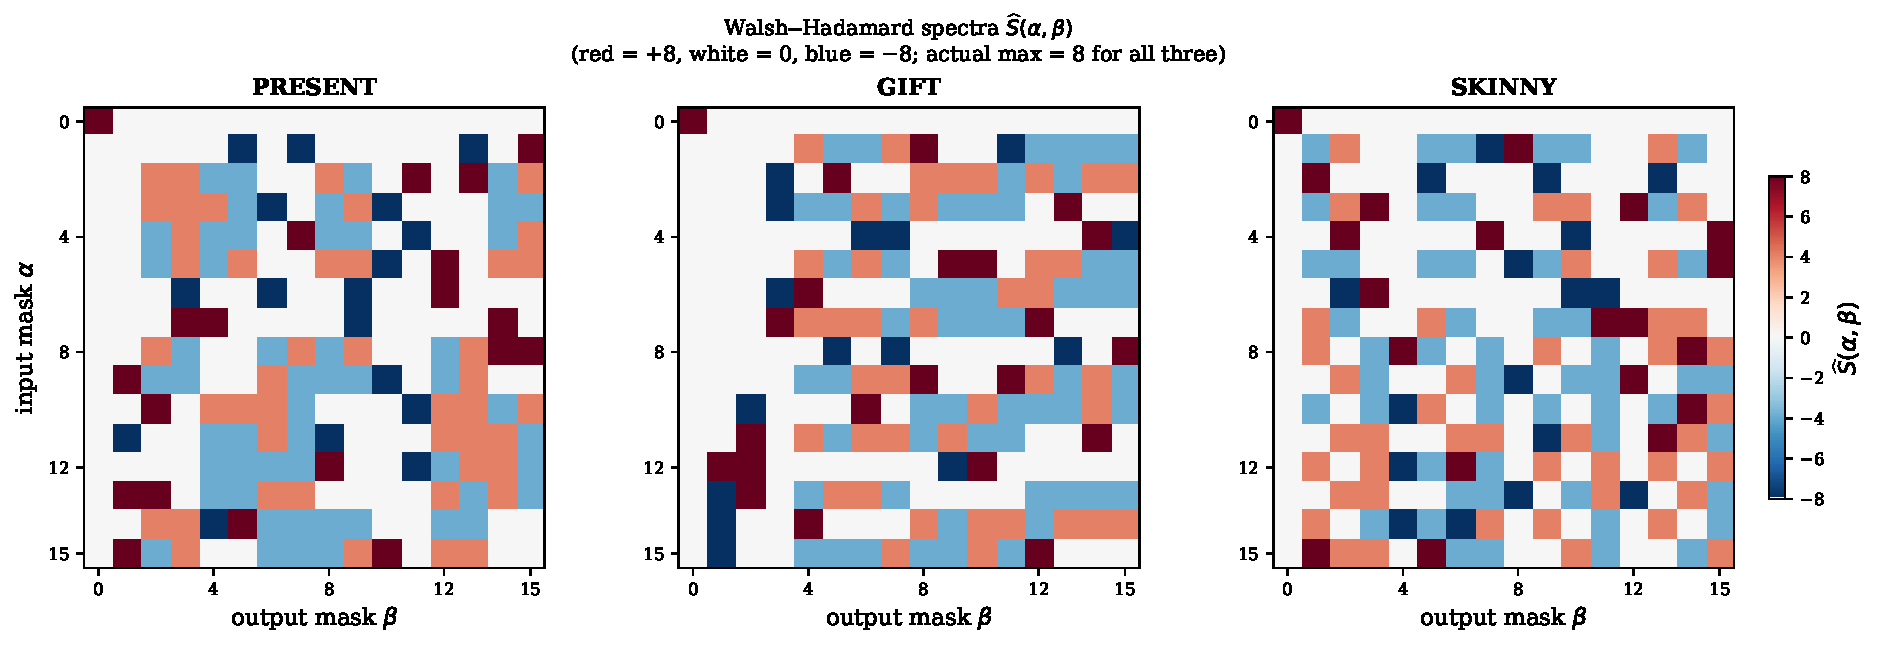
\includegraphics[width=\textwidth]{fig1_wht_spectra.pdf}
\caption{Walsh spectra. The plotted Walsh tables show the same amplitude
profile for PRESENT, GIFT, and SKINNY, which explains why purely
amplitude-based diagnostics coincide for these examples.}
\label{fig:wht-spectra}
\end{figure}

\begin{figure}[t]
\centering
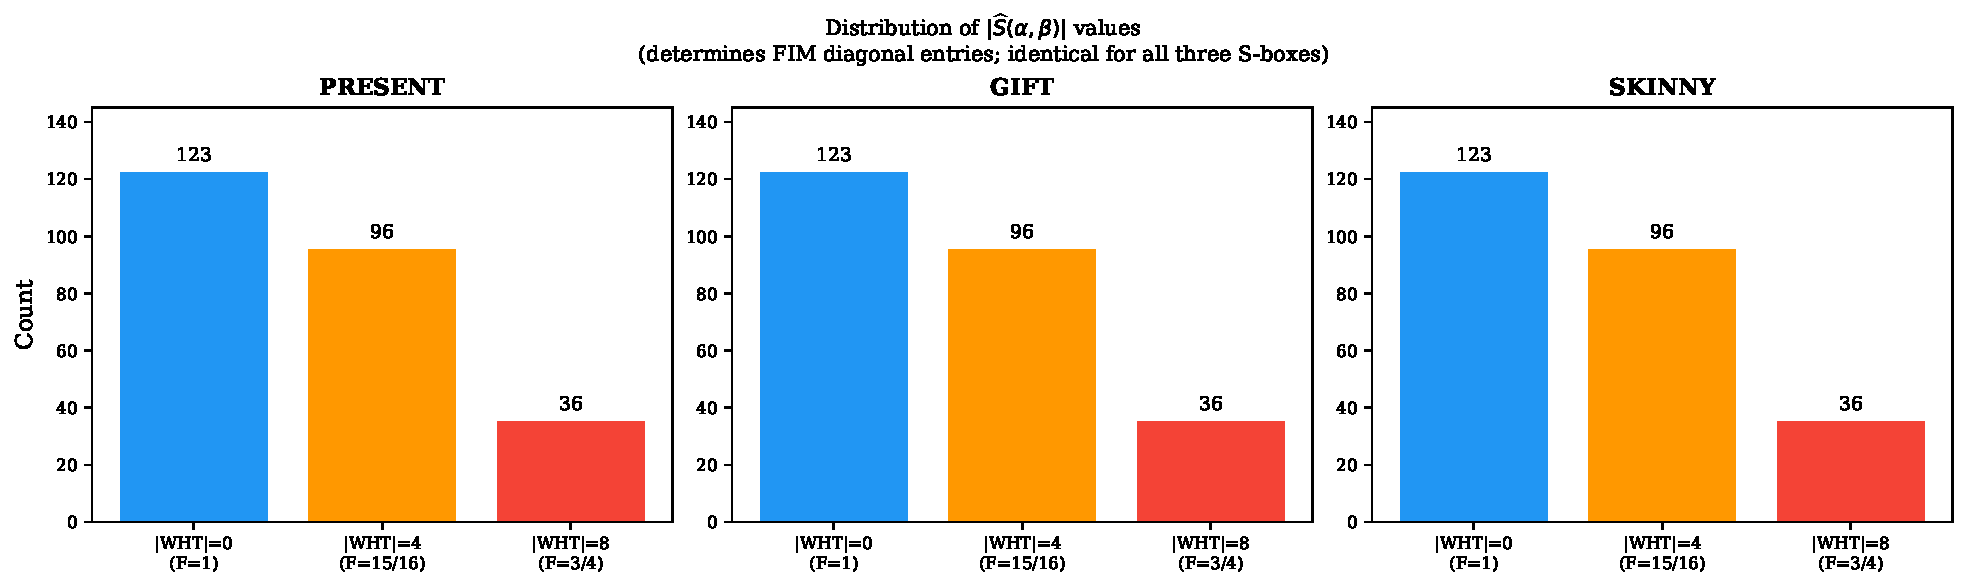
\includegraphics[width=0.74\textwidth]{fig2_wht_histogram.pdf}
\caption{Walsh amplitude distribution. The histogram records the shared counts
of absolute Walsh coefficients over nonzero masks for the three tested S-boxes.}
\label{fig:wht-histogram}
\end{figure}

The boundary covariance matrix is built from Proposition~\ref{thm:fim}.  For
$s=4$ it is a $255\times255$ positive semidefinite matrix.  Consistent with
Theorem~\ref{thm:active-rank}, all three matrices have rank $15$ and active
eigenvalues equal to $16$ up to numerical precision.

\begin{table}[t]
\centering
\caption{Boundary covariance structure for the tested 4-bit bijections.}
\label{tab:cov-rank}
\begin{tabular}{lccc}
\toprule
S-box & Matrix size & Rank & Active eigenvalues \\
\midrule
PRESENT & $255\times255$ & $15$ & $16$ repeated $15$ times \\
GIFT    & $255\times255$ & $15$ & $16$ repeated $15$ times \\
SKINNY  & $255\times255$ & $15$ & $16$ repeated $15$ times \\
\bottomrule
\end{tabular}
\end{table}

\subsection{Local spectral separation}\label{subsec:fr-distances}

Using~\eqref{eq:fr-local}, we compute local diagonal Walsh/Fisher separation
proxies between key hypotheses.  This local covariance-weighted coordinate
displacement is evaluated in the regularized Walsh/Fisher coordinates
introduced earlier.  The key-translation rule implies that the value depends
only on the key difference $k\oplus k'$.

\begin{figure}[t]
\centering
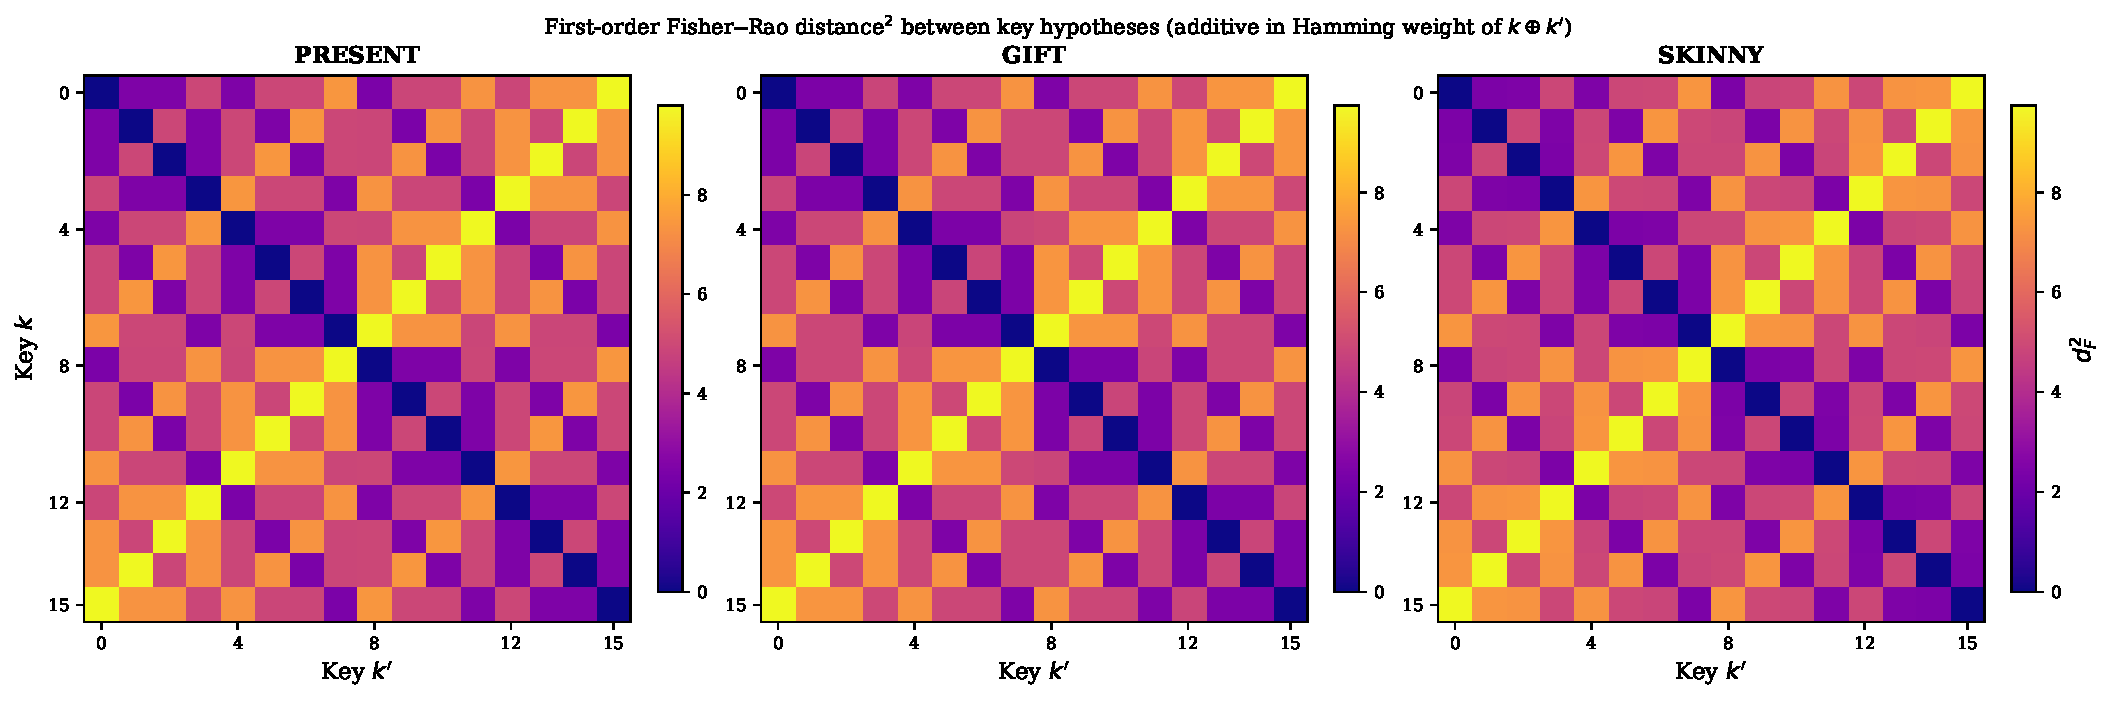
\includegraphics[width=0.8\textwidth]{fig3_fr_distance_matrix.pdf}
\caption{Local key-separation proxy. The matrix visualises the
covariance-weighted Walsh displacement between key hypotheses in the local
Walsh/Fisher coordinates.}
\label{fig:local-distance}
\end{figure}

\begin{figure}[t]
\centering
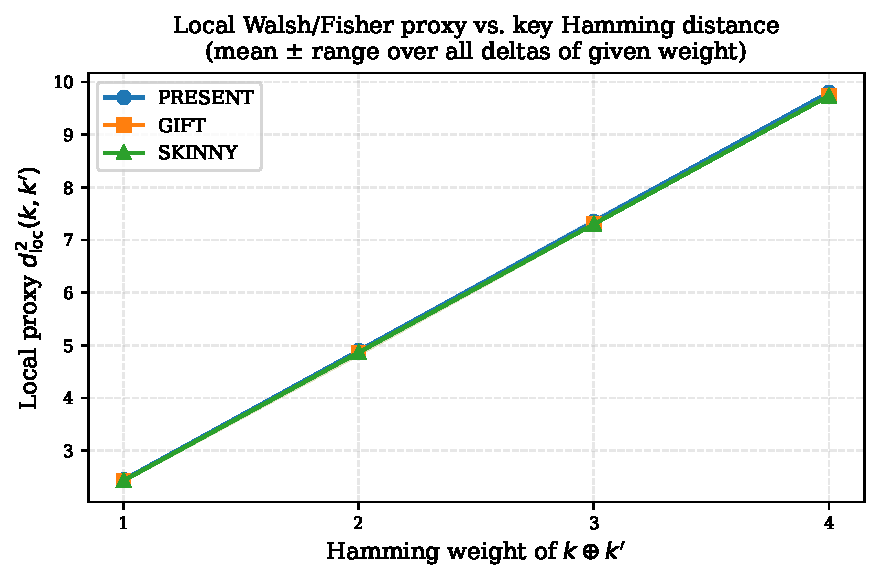
\includegraphics[width=0.74\textwidth]{fig5_fr_vs_hw.pdf}
\caption{Local proxy versus key-difference Hamming weight.  The plot aggregates
the same covariance-weighted Walsh displacement by the Hamming weight of
$k\oplus k'$.}
\label{fig:local-distance-hw}
\end{figure}

\begin{table}[t]
\centering
\caption{Interpretation of the key-separation quantities.}
\label{tab:distance-status}
\begin{tabular}{ll}
\toprule
Quantity & Status \\
\midrule
$\KL(P_k\|P_{k'})$ for $k\neq k'$ & Infinite, because supports are disjoint \\
$d_F(\delta_k,\delta_{k'})$ on the belief simplex & Exactly $\pi$ \\
$d_{\mathrm{loc}}^2(k,k')$ in~\eqref{eq:fr-local} & Local Walsh/Fisher covariance proxy \\
\bottomrule
\end{tabular}
\end{table}

\subsection{CPA leakage gaps}\label{subsec:pairwise-gap-numerical}

For bijective 4-bit S-boxes and uniform inputs, the scalar Hamming-weight
variance in Proposition~\ref{thm:per-trace} is always
\[
  I_S(\HW,\sigma)=\frac{1}{\sigma^2}.
\]
This scalar is a baseline leakage descriptor shared by PRESENT, GIFT, and
SKINNY.  Pairwise gaps
\[
  \Delta(\delta)=\frac1{16}\sum_{a\in\B{4}}
  \bigl(\HW(S(a))-\HW(S(a\oplus\delta))\bigr)^2,
  \qquad \delta\neq0,
\]
are more informative for CPA because the expected log-Bayes gain against a
wrong key with difference $\delta$ is $\Delta(\delta)/(2\sigma^2)$.

\begin{table}[t]
\centering
\caption{Pairwise Hamming-weight leakage gaps over nonzero key differences.}
\label{tab:pairwise-gaps}
\begin{tabular}{lccc}
\toprule
S-box & $\min_{\delta\neq0}\Delta(\delta)$ &
$\max_{\delta\neq0}\Delta(\delta)$ &
$\frac1{15}\sum_{\delta\neq0}\Delta(\delta)$ \\
\midrule
PRESENT & $1$ & $7/2$ & $32/15$ \\
GIFT    & $5/4$ & $7/2$ & $32/15$ \\
SKINNY  & $1$ & $3$   & $32/15$ \\
\bottomrule
\end{tabular}
\end{table}

Table~\ref{tab:pairwise-gaps} shows how the scalar variance descriptor and the
pairwise structure play complementary roles: all three S-boxes have the same
average pairwise gap, while the worst and best key-difference cases vary.
These pairwise gaps are the
quantities that enter expected posterior-odds growth in the Gaussian leakage
model.

\begin{table}[t]
\centering
\caption{Operational CPA interpretation of the pairwise gaps.  The listed
deltas are nonzero key differences $\delta=k\oplus k^*$ in hexadecimal.}
\label{tab:gap-distribution}
\scriptsize
\setlength{\tabcolsep}{2pt}
\begin{tabular}{@{}p{0.13\textwidth}p{0.17\textwidth}p{0.17\textwidth}p{0.43\textwidth}@{}}
\toprule
S-box & Hardest gaps $\min\Delta$ & Easiest gaps $\max\Delta$ &
Gap multiset over $\delta\neq0$ \\
\midrule
PRESENT & $1$ at $\{A,E\}$ & $7/2$ at $\{6\}$ &
$1^2$; $(5/4)^1$; $(3/2)^2$; $(7/4)^3$; $(5/2)^2$;
$(11/4)^1$; $3^2$; $(13/4)^1$; $(7/2)^1$ \\
GIFT & $5/4$ at $\{C,E,F\}$ & $7/2$ at $\{7\}$ &
$(5/4)^3$; $(3/2)^2$; $2^2$; $(9/4)^3$; $(5/2)^2$;
$3^2$; $(7/2)^1$ \\
SKINNY & $1$ at $\{5\}$ & $3$ at $\{B\}$ &
$1^1$; $(5/4)^1$; $(3/2)^1$; $(7/4)^1$; $2^3$;
$(9/4)^2$; $(5/2)^3$; $(11/4)^2$; $3^1$ \\
\bottomrule
\end{tabular}
\end{table}

Table~\ref{tab:gap-distribution} gives the CPA-oriented reading of the
pairwise theory.  PRESENT and SKINNY have a smaller hardest-key gap than GIFT
under this leakage model, so the model-based estimate
\eqref{eq:gap-sample-estimate} assigns a larger trace budget to the hardest
posterior-odds margin for those S-boxes.  The comparison is local to the
specified S-box computation and leakage model, which is the level at which CPA
key hypotheses are evaluated.

\subsection{Monte Carlo CPA validation}\label{subsec:cpa-simulation}

To connect the gap analysis to an attack observable, we simulate the Bayesian
CPA model of Section~\ref{sec:cpa}.  For each S-box, we use true key
$k^*=0$, uniformly sampled plaintext nibbles, leakage
$W=\HW(S(a\oplus k^*))+\varepsilon$, Gaussian noise standard deviation
$\sigma=2$, and $3000$ Monte Carlo trials with seed $20260622$.  For every
trace prefix, all 16 key log-likelihoods are accumulated and the true-key rank
is recorded.  The script \texttt{simulate\_cpa.py} regenerates both
Fig.~\ref{fig:cpa-simulation} and the CSV summary
\texttt{cpa\_simulation\_results.csv}.

\begin{figure}[t]
\centering
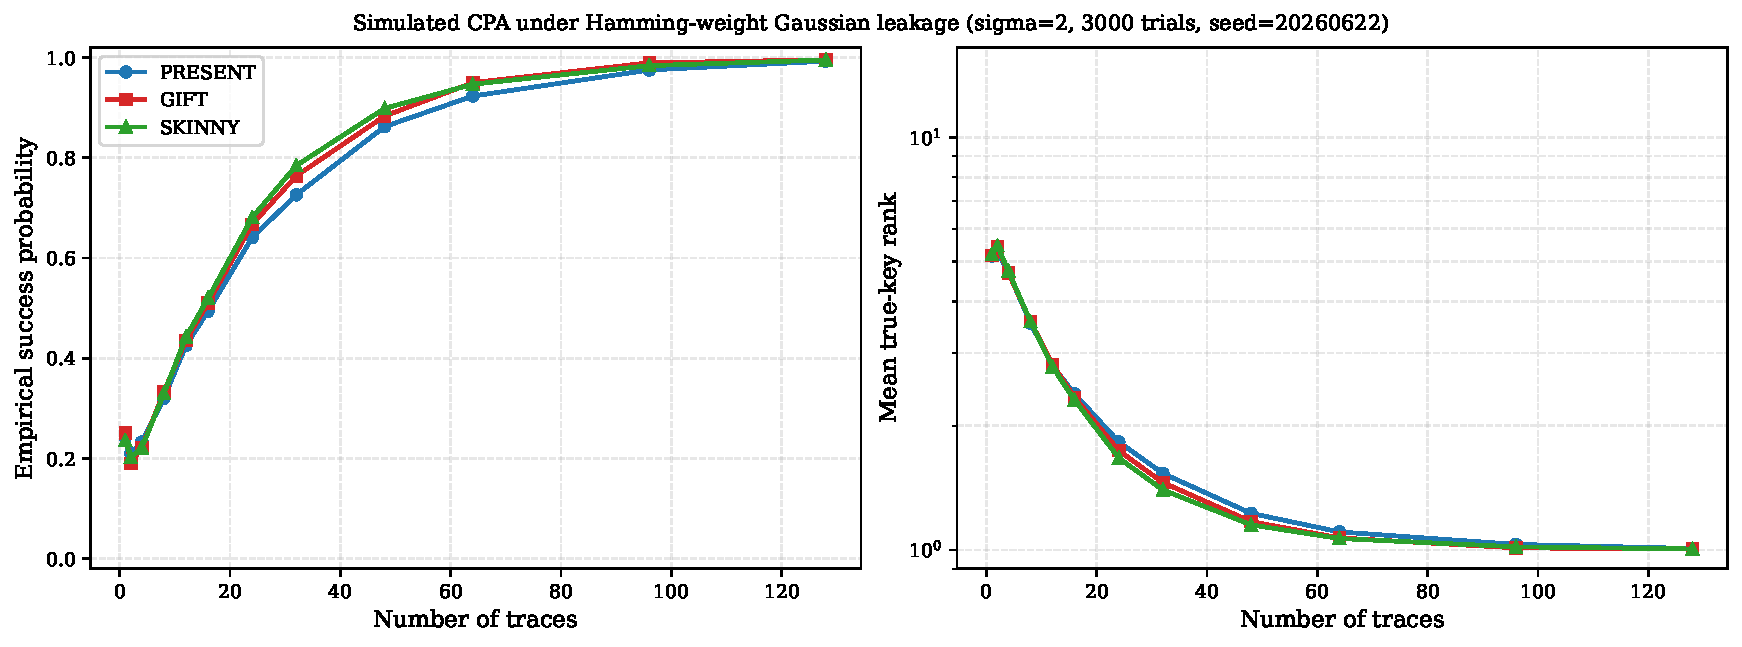
\includegraphics[width=\textwidth]{fig6_cpa_simulation.pdf}
\caption{Simulated CPA under Hamming-weight Gaussian leakage.  The left panel
shows empirical success probability and the right panel shows mean true-key
rank over $3000$ trials.  The curves translate the pairwise-gap analysis into
trace-dependent attack observables.}
\label{fig:cpa-simulation}
\end{figure}

The simulation confirms the qualitative role of the pairwise gaps.  At
$64$ traces, the empirical success probabilities are approximately $0.923$ for
PRESENT, $0.950$ for GIFT, and $0.947$ for SKINNY; at $128$ traces, all three
success probabilities are between $0.993$ and $0.996$.  Mean true-key ranks
decrease toward one for all three S-boxes.  The finite-trace curves summarize
the combined effect of all wrong-key competitors, while the minimum gap in
Table~\ref{tab:pairwise-gaps} controls the hardest pairwise posterior-odds
growth.

\begin{figure}[t]
\centering
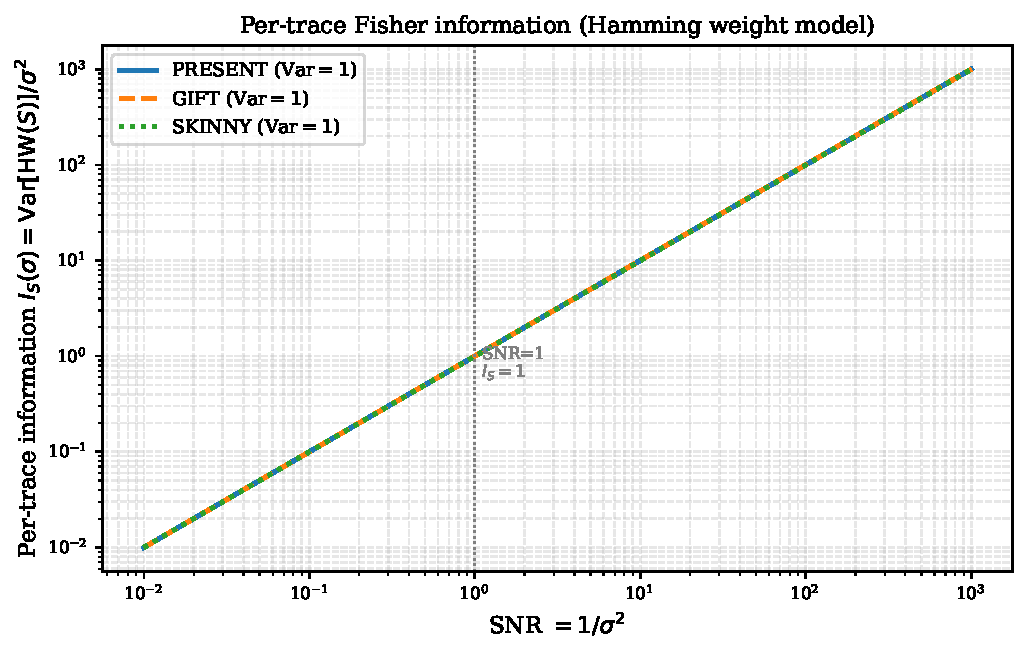
\includegraphics[width=0.74\textwidth]{fig4_per_trace_info.pdf}
\caption{Per-trace leakage baseline. The scalar Hamming-weight variance is the
same for all bijective 4-bit S-boxes under uniform inputs, so CPA discrimination
is completed by pairwise leakage gaps that determine key-hypothesis
discrimination.}
\label{fig:per-trace-info}
\end{figure}

\subsection{Active-eigenspace curvature}\label{subsec:curv-numerical}

The curvature diagnostic of Section~\ref{sec:curvature} is evaluated in the
15-dimensional active eigenspace of the boundary covariance matrix.  The result
is constant for all coordinate planes in the tested cases.

\begin{table}[t]
\centering
\caption{Projected active-eigenspace curvature diagnostic for the tested 4-bit S-boxes.}
\label{tab:curvatures}
\begin{tabular}{lcccc}
\toprule
S-box & Active dimension & Planes & Min $K$ & Max $K$ \\
\midrule
PRESENT & $15$ & $105$ & $-0.25$ & $-0.25$ \\
GIFT    & $15$ & $105$ & $-0.25$ & $-0.25$ \\
SKINNY  & $15$ & $105$ & $-0.25$ & $-0.25$ \\
\bottomrule
\end{tabular}
\end{table}

\subsection{Reproducibility checklist}\label{subsec:repro-checklist}

The computational claims in this section are reproducible from the additional
files.  The scripts \texttt{gen\_figures.py}, \texttt{simulate\_cpa.py},
\texttt{compute\_curvatures.py}, and \texttt{verify\_curvature.py} regenerate
the figures, CPA simulation results, active covariance diagnostics, and
curvature checks.  The
rank/eigenvalue statement is proved independently in
Theorem~\ref{thm:active-rank}; the scripts provide finite checks for the
reported 4-bit examples.

% ============================================================================
% End inlined file: sections/numerical.tex
% ============================================================================
% ============================================================================
% Begin inlined file: sections/discussion.tex
% ============================================================================
% ============================================================================
% SECTION 8: DISCUSSION
% ============================================================================
\section{Discussion}\label{sec:discussion}

\subsection{What the framework establishes}

The framework establishes a controlled information-geometric model for the
local S-box distributions that appear in side-channel key recovery.  Its first
role is structural: exact key-induced distributions are singular boundary
points, while ordinary Fisher--Rao geometry belongs to full-support interiors
or to the adversary's belief simplex.  This distinction prevents assigning
non-degenerate Fisher metrics, finite KL divergences, or ordinary geodesics to
disjoint-support key endpoints.

The second role is algebraic.  Walsh characters give explicit coordinates for
the boundary orbit, and the key-translation rule determines how expectation
coordinates move when the key hypothesis changes.  This rule is elementary,
but it is useful because it gives closed-form covariance and displacement
expressions.

The third role is security-oriented.  CPA is a Bayesian trajectory on the
belief simplex.  Under the Gaussian leakage model, pairwise Hamming-weight gaps
determine expected log-Bayes gains against wrong keys.  The scalar leakage
variance is therefore a baseline descriptor, whereas pairwise gaps describe
the discrimination structure relevant to key recovery.

This gives a concrete review criterion for the proposed quantities.  A
diagnostic is useful for side-channel security when it changes the
interpretation of posterior-odds growth, hard key differences, or the validity
of a geometric approximation.  The numerical section combines the shared
Walsh-amplitude invariants of PRESENT, GIFT, and SKINNY with the pairwise gap
distributions and simulated CPA curves that determine which wrong keys are
hardest to eliminate under the stated leakage model.

\subsection{Position within S-box and side-channel analysis}

The framework uses established 4-bit S-box classifications as background and
focuses on the local distributions used in side-channel key recovery.  PRESENT,
GIFT, and SKINNY serve as reproducible lightweight examples with shared
Walsh-amplitude profiles and different CPA gap distributions.  The standard
Gaussian Hamming-weight CPA model provides the inference setting in which the
boundary S-box law, posterior belief law, and pairwise discrimination gaps are
connected.

\subsection{Cryptographic interpretation}

For isolated bijective 4-bit S-boxes under uniform input and Hamming-weight
leakage, $I_S(\HW,\sigma)=1/\sigma^2$ for every bijection.  This equality is
best used as a baseline descriptor.  Practical side-channel behavior is shaped
by pairwise leakage gaps, implementation leakage, noise, masking, alignment,
higher-order effects, and the full cipher context.

In this sense, identical Walsh-amplitude histograms are a useful baseline.
They show which quantities are shared by the three tested S-boxes, while the
CPA gap distribution and Monte Carlo curves expose model-dependent hard and
easy key differences.  This is precisely the separation required before using
information-geometric language in a cybersecurity setting.

The boundary covariance and local Walsh/Fisher separation proxy complement LAT,
DDT, and empirical leakage evaluation.  They provide coordinate diagnostics
for the singular key orbit and inputs to posterior belief dynamics alongside
standard cryptanalytic criteria.

\subsection{Status of the curvature finding}

The active-eigenspace value \(K=-1/4\) is reported as a reproducible diagnostic
under the projection, normalization, and sign conventions specified in
Section~\ref{sec:curvature}.  The rank and active eigenvalue statement is
proved for every bijective S-box.  A complete symbolic characterization of the
curvature diagnostic, including the exact hypotheses under which it is
constant, remains open.

\subsection{Open problems}\label{subsec:extensions}

Several extensions are natural.  First, the $\varepsilon\downarrow0$ limit of
regularized Fisher--Rao geometry could be studied using tools from singular
information geometry.  Second, the active-eigenspace curvature phenomenon
could be attacked symbolically.  Third, the leakage model could be extended to
masked, higher-order, non-Gaussian, or profiled settings.  Fourth, full-round
ciphers can be handled by adding propagation through linear layers and key
schedules.

% ============================================================================
% End inlined file: sections/discussion.tex
% ============================================================================
% ============================================================================
% Begin inlined file: sections/conclusion.tex
% ============================================================================
% ============================================================================
% SECTION 9: CONCLUSION
% ============================================================================
\section{Conclusion}\label{sec:conclusion}

We presented a boundary information-geometric framework for the local S-box
distributions that arise in side-channel key recovery.  The main modelling
point is the separation between three spaces: the regular full-support Walsh
exponential family, the singular key-induced boundary orbit, and the
adversary's belief simplex.  This separation makes Fisher, KL, and projection
statements mathematically well scoped.

For bijective S-boxes, Walsh coordinates give closed-form boundary covariance
matrices.  The active covariance subspace has dimension $2^s-1$ and all active
eigenvalues equal $2^s$ in the unnormalised Walsh basis.  Thus this part of the
geometry is a general structural consequence of bijectivity.

For CPA, Bayesian updates occur on the belief simplex.  Under Hamming-weight
Gaussian leakage, the scalar variance information is a baseline fixed by
bijectivity, while pairwise leakage gaps determine expected posterior-odds
growth against wrong keys.  Computations on PRESENT, GIFT, and SKINNY
illustrate this distinction and reproduce the active curvature diagnostic
$K=-1/4$ in the tested 4-bit cases.

The framework contributes a controlled geometric language for connecting
singular S-box distributions, boundary covariance, and side-channel Bayesian
inference.
The security value of the framework is to make explicit which geometric
quantities are structural invariants and which quantities affect local
key-hypothesis discrimination under a specified leakage model.

% ============================================================================
% End inlined file: sections/conclusion.tex
% ============================================================================
% ============================================================================
% Begin inlined file: appendices/reproducibility_ano.tex
% ============================================================================
% ============================================================================
% DECLARATIONS FOR THE BLINDED MANUSCRIPT
% ============================================================================
\section*{Declarations}

\subsection*{Availability of data and material}

The datasets supporting the conclusions of this article are included within the
article and its additional files. Additional file 1,
\texttt{supplementary\_reproducibility.pdf}, records the computational
protocol, software environment, arithmetic conventions, and reproducibility
coverage. Additional file 2, \texttt{supplementary\_material.zip}, contains
the scripts, dependency list, CPA simulation CSV, and reproduction README used
to regenerate the numerical tables and figures.

Software information: project name, Boundary Information Geometry for S-box
Side-Channel Leakage; project home page,
\url{https://anonymous.4open.science/r/IG-based-Sbox-SCL-DE49/};
operating system, platform independent; programming language, Python 3; other
requirements, \texttt{numpy}, \texttt{scipy}, and \texttt{matplotlib};
license, not specified; restrictions to use by non-academics, none beyond the
repository license status.

\subsection*{Funding}

Not applicable.

\subsection*{Acknowledgements}

Not applicable.

% ============================================================================
% End inlined file: appendices/reproducibility_ano.tex
% ============================================================================

% ============================================================================
%% BioMed_Central_Bib_Style_v1.01

\begin{thebibliography}{15}
% BibTex style file: bmc-mathphys.bst (version 2.1), 2014-07-24
\ifx \bisbn   \undefined \def \bisbn  #1{ISBN #1}\fi
\ifx \binits  \undefined \def \binits#1{#1}\fi
\ifx \bauthor  \undefined \def \bauthor#1{#1}\fi
\ifx \batitle  \undefined \def \batitle#1{#1}\fi
\ifx \bjtitle  \undefined \def \bjtitle#1{#1}\fi
\ifx \bvolume  \undefined \def \bvolume#1{\textbf{#1}}\fi
\ifx \byear  \undefined \def \byear#1{#1}\fi
\ifx \bissue  \undefined \def \bissue#1{#1}\fi
\ifx \bfpage  \undefined \def \bfpage#1{#1}\fi
\ifx \blpage  \undefined \def \blpage #1{#1}\fi
\ifx \burl  \undefined \def \burl#1{\textsf{#1}}\fi
\ifx \doiurl  \undefined \def \doiurl#1{\url{https://doi.org/#1}}\fi
\ifx \betal  \undefined \def \betal{\textit{et al.}}\fi
\ifx \binstitute  \undefined \def \binstitute#1{#1}\fi
\ifx \binstitutionaled  \undefined \def \binstitutionaled#1{#1}\fi
\ifx \bctitle  \undefined \def \bctitle#1{#1}\fi
\ifx \beditor  \undefined \def \beditor#1{#1}\fi
\ifx \bpublisher  \undefined \def \bpublisher#1{#1}\fi
\ifx \bbtitle  \undefined \def \bbtitle#1{#1}\fi
\ifx \bedition  \undefined \def \bedition#1{#1}\fi
\ifx \bseriesno  \undefined \def \bseriesno#1{#1}\fi
\ifx \blocation  \undefined \def \blocation#1{#1}\fi
\ifx \bsertitle  \undefined \def \bsertitle#1{#1}\fi
\ifx \bsnm \undefined \def \bsnm#1{#1}\fi
\ifx \bsuffix \undefined \def \bsuffix#1{#1}\fi
\ifx \bparticle \undefined \def \bparticle#1{#1}\fi
\ifx \barticle \undefined \def \barticle#1{#1}\fi
\bibcommenthead
\ifx \bconfdate \undefined \def \bconfdate #1{#1}\fi
\ifx \botherref \undefined \def \botherref #1{#1}\fi
\ifx \url \undefined \def \url#1{\textsf{#1}}\fi
\ifx \bchapter \undefined \def \bchapter#1{#1}\fi
\ifx \bbook \undefined \def \bbook#1{#1}\fi
\ifx \bcomment \undefined \def \bcomment#1{#1}\fi
\ifx \oauthor \undefined \def \oauthor#1{#1}\fi
\ifx \citeauthoryear \undefined \def \citeauthoryear#1{#1}\fi
\ifx \endbibitem  \undefined \def \endbibitem {}\fi
\ifx \bconflocation  \undefined \def \bconflocation#1{#1}\fi
\ifx \arxivurl  \undefined \def \arxivurl#1{\textsf{#1}}\fi
\csname PreBibitemsHook\endcsname

%%% 1
\bibitem[\protect\citeauthoryear{ichi Amari and
  Nagaoka}{2000}]{amari2000methods}
\begin{bbook}
\bauthor{\bsnm{Amari}, \binits{S.-i.}},
\bauthor{\bsnm{Nagaoka}, \binits{H.}}:
\bbtitle{Methods of Information Geometry}.
\bsertitle{Translations of Mathematical Monographs},
vol. \bseriesno{191}.
\bpublisher{American Mathematical Society / Oxford University Press},
\blocation{Providence, RI / Oxford}
(\byear{2000}).
\bcomment{Translated by Daishi Harada}
\end{bbook}
\endbibitem

%%% 2
\bibitem[\protect\citeauthoryear{Ay et~al.}{2017}]{ay2017information}
\begin{bbook}
\bauthor{\bsnm{Ay}, \binits{N.}},
\bauthor{\bsnm{Jost}, \binits{J.}},
\bauthor{\bsnm{L{\^e}}, \binits{H.V.}},
\bauthor{\bsnm{Schwachh{\"o}fer}, \binits{L.}}:
\bbtitle{Information Geometry}.
\bsertitle{Ergebnisse der Mathematik und ihrer Grenzgebiete}.
\bpublisher{Springer},
\blocation{Cham}
(\byear{2017})
\end{bbook}
\endbibitem

%%% 3
\bibitem[\protect\citeauthoryear{Chentsov}{1982}]{chentsov1982statistical}
\begin{bbook}
\bauthor{\bsnm{Chentsov}, \binits{N.N.}}:
\bbtitle{Statistical Decision Rules and Optimal Inference}.
\bsertitle{Translations of Mathematical Monographs},
vol. \bseriesno{53}.
\bpublisher{American Mathematical Society},
\blocation{Providence, RI}
(\byear{1982})
\end{bbook}
\endbibitem

%%% 4
\bibitem[\protect\citeauthoryear{Ikeda et~al.}{2004}]{ikeda2004information}
\begin{barticle}
\bauthor{\bsnm{Ikeda}, \binits{S.}},
\bauthor{\bsnm{Tanaka}, \binits{T.}},
\bauthor{\bsnm{Amari}, \binits{S.-i.}}:
\batitle{Information geometry of turbo and low-density parity-check codes}.
\bjtitle{IEEE Transactions on Information Theory}
\bvolume{50}(\bissue{6}),
\bfpage{1097}--\blpage{1114}
(\byear{2004})
\doiurl{10.1109/TIT.2004.828072}
\end{barticle}
\endbibitem

%%% 5
\bibitem[\protect\citeauthoryear{Nyberg}{1994}]{nyberg1994differentially}
\begin{bchapter}
\bauthor{\bsnm{Nyberg}, \binits{K.}}:
\bctitle{Differentially uniform mappings for cryptography}.
In: \bbtitle{Advances in Cryptology -- EUROCRYPT 1993}.
\bsertitle{Lecture Notes in Computer Science},
vol. \bseriesno{765},
pp. \bfpage{55}--\blpage{64}.
\bpublisher{Springer},
\blocation{Berlin, Heidelberg}
(\byear{1994}).
\doiurl{10.1007/3-540-48285-7_6}
\end{bchapter}
\endbibitem

%%% 6
\bibitem[\protect\citeauthoryear{Leander and
  Poschmann}{2007}]{leander2007classification}
\begin{bchapter}
\bauthor{\bsnm{Leander}, \binits{G.}},
\bauthor{\bsnm{Poschmann}, \binits{A.}}:
\bctitle{On the classification of 4 bit {S}-boxes}.
In: \bbtitle{Arithmetic of Finite Fields -- WAIFI 2007}.
\bsertitle{Lecture Notes in Computer Science},
vol. \bseriesno{4547},
pp. \bfpage{159}--\blpage{176}.
\bpublisher{Springer},
\blocation{Berlin, Heidelberg}
(\byear{2007}).
\doiurl{10.1007/978-3-540-73074-3_13}
\end{bchapter}
\endbibitem

%%% 7
\bibitem[\protect\citeauthoryear{Beyne}{2021}]{beyne2021geometric}
\begin{bchapter}
\bauthor{\bsnm{Beyne}, \binits{T.}}:
\bctitle{A geometric approach to linear cryptanalysis}.
In: \bbtitle{Advances in Cryptology -- ASIACRYPT 2021}.
\bsertitle{Lecture Notes in Computer Science},
vol. \bseriesno{13090},
pp. \bfpage{36}--\blpage{66}.
\bpublisher{Springer},
\blocation{Cham}
(\byear{2021}).
\doiurl{10.1007/978-3-030-92068-5_2}
\end{bchapter}
\endbibitem

%%% 8
\bibitem[\protect\citeauthoryear{Beyne and
  Rijmen}{2022}]{beyne2022quasidifferential}
\begin{bchapter}
\bauthor{\bsnm{Beyne}, \binits{T.}},
\bauthor{\bsnm{Rijmen}, \binits{V.}}:
\bctitle{Differential cryptanalysis in the fixed-key model}.
In: \bbtitle{Advances in Cryptology -- CRYPTO 2022}.
\bsertitle{Lecture Notes in Computer Science},
vol. \bseriesno{13509},
pp. \bfpage{687}--\blpage{716}.
\bpublisher{Springer},
\blocation{Cham}
(\byear{2022}).
\doiurl{10.1007/978-3-031-15982-4_23}
\end{bchapter}
\endbibitem

%%% 9
\bibitem[\protect\citeauthoryear{Kocher et~al.}{1999}]{kocher1999differential}
\begin{bchapter}
\bauthor{\bsnm{Kocher}, \binits{P.}},
\bauthor{\bsnm{Jaffe}, \binits{J.}},
\bauthor{\bsnm{Jun}, \binits{B.}}:
\bctitle{Differential power analysis}.
In: \bbtitle{Advances in Cryptology -- CRYPTO 1999}.
\bsertitle{Lecture Notes in Computer Science},
vol. \bseriesno{1666},
pp. \bfpage{388}--\blpage{397}.
\bpublisher{Springer},
\blocation{Berlin, Heidelberg}
(\byear{1999}).
\doiurl{10.1007/3-540-48405-1_25}
\end{bchapter}
\endbibitem

%%% 10
\bibitem[\protect\citeauthoryear{Brier et~al.}{2004}]{brier2004correlation}
\begin{bchapter}
\bauthor{\bsnm{Brier}, \binits{E.}},
\bauthor{\bsnm{Clavier}, \binits{C.}},
\bauthor{\bsnm{Olivier}, \binits{F.}}:
\bctitle{Correlation power analysis with a leakage model}.
In: \bbtitle{Cryptographic Hardware and Embedded Systems -- CHES 2004}.
\bsertitle{Lecture Notes in Computer Science},
vol. \bseriesno{3156},
pp. \bfpage{16}--\blpage{29}.
\bpublisher{Springer},
\blocation{Berlin, Heidelberg}
(\byear{2004}).
\doiurl{10.1007/978-3-540-28632-5_2}
\end{bchapter}
\endbibitem

%%% 11
\bibitem[\protect\citeauthoryear{Standaert et~al.}{2009}]{standaert2009unified}
\begin{bchapter}
\bauthor{\bsnm{Standaert}, \binits{F.-X.}},
\bauthor{\bsnm{Malkin}, \binits{T.G.}},
\bauthor{\bsnm{Yung}, \binits{M.}}:
\bctitle{A unified framework for the analysis of side-channel key recovery
  attacks}.
In: \bbtitle{Advances in Cryptology -- EUROCRYPT 2009}.
\bsertitle{Lecture Notes in Computer Science},
vol. \bseriesno{5479},
pp. \bfpage{443}--\blpage{461}.
\bpublisher{Springer},
\blocation{Berlin, Heidelberg}
(\byear{2009}).
\doiurl{10.1007/978-3-642-01001-9_26}
\end{bchapter}
\endbibitem

%%% 12
\bibitem[\protect\citeauthoryear{Veyrat-Charvillon and
  Standaert}{2009}]{veyrat2009adaptive}
\begin{bchapter}
\bauthor{\bsnm{Veyrat-Charvillon}, \binits{N.}},
\bauthor{\bsnm{Standaert}, \binits{F.-X.}}:
\bctitle{Mutual information analysis: How, when and why?}
In: \bbtitle{Cryptographic Hardware and Embedded Systems -- CHES 2009}.
\bsertitle{Lecture Notes in Computer Science},
vol. \bseriesno{5747},
pp. \bfpage{429}--\blpage{443}.
\bpublisher{Springer},
\blocation{Berlin, Heidelberg}
(\byear{2009}).
\doiurl{10.1007/978-3-642-04138-9_30}
\end{bchapter}
\endbibitem

%%% 13
\bibitem[\protect\citeauthoryear{Bogdanov et~al.}{2007}]{bogdanov2007present}
\begin{bchapter}
\bauthor{\bsnm{Bogdanov}, \binits{A.}},
\bauthor{\bsnm{Knudsen}, \binits{L.R.}},
\bauthor{\bsnm{Leander}, \binits{G.}},
\bauthor{\bsnm{Paar}, \binits{C.}},
\bauthor{\bsnm{Poschmann}, \binits{A.}},
\bauthor{\bsnm{Robshaw}, \binits{M.J.B.}},
\bauthor{\bsnm{Seurin}, \binits{Y.}},
\bauthor{\bsnm{Vikkelsoe}, \binits{C.}}:
\bctitle{{PRESENT}: An ultra-lightweight block cipher}.
In: \bbtitle{Cryptographic Hardware and Embedded Systems -- CHES 2007}.
\bsertitle{Lecture Notes in Computer Science},
vol. \bseriesno{4727},
pp. \bfpage{450}--\blpage{466}.
\bpublisher{Springer},
\blocation{Berlin, Heidelberg}
(\byear{2007}).
\doiurl{10.1007/978-3-540-74735-2_31}
\end{bchapter}
\endbibitem

%%% 14
\bibitem[\protect\citeauthoryear{Banik et~al.}{2017}]{banik2017gift}
\begin{bchapter}
\bauthor{\bsnm{Banik}, \binits{S.}},
\bauthor{\bsnm{Pandey}, \binits{S.K.}},
\bauthor{\bsnm{Peyrin}, \binits{T.}},
\bauthor{\bsnm{Sasaki}, \binits{Y.}},
\bauthor{\bsnm{Sim}, \binits{S.M.}},
\bauthor{\bsnm{Todo}, \binits{Y.}}:
\bctitle{{GIFT}: A small present -- towards reaching the limit of lightweight
  encryption}.
In: \bbtitle{Cryptographic Hardware and Embedded Systems -- CHES 2017}.
\bsertitle{Lecture Notes in Computer Science},
vol. \bseriesno{10529},
pp. \bfpage{321}--\blpage{345}.
\bpublisher{Springer},
\blocation{Cham}
(\byear{2017}).
\doiurl{10.1007/978-3-319-66787-4_16}
\end{bchapter}
\endbibitem

%%% 15
\bibitem[\protect\citeauthoryear{Beierle et~al.}{2016}]{beierle2016skinny}
\begin{bchapter}
\bauthor{\bsnm{Beierle}, \binits{C.}},
\bauthor{\bsnm{Jean}, \binits{J.}},
\bauthor{\bsnm{K{\"o}lbl}, \binits{S.}},
\bauthor{\bsnm{Leander}, \binits{G.}},
\bauthor{\bsnm{Moradi}, \binits{A.}},
\bauthor{\bsnm{Peyrin}, \binits{T.}},
\bauthor{\bsnm{Sasaki}, \binits{Y.}},
\bauthor{\bsnm{Sasdrich}, \binits{P.}},
\bauthor{\bsnm{Sim}, \binits{S.M.}}:
\bctitle{The {SKINNY} family of block ciphers and its low-latency variant
  {MANTIS}}.
In: \bbtitle{Advances in Cryptology -- CRYPTO 2016}.
\bsertitle{Lecture Notes in Computer Science},
vol. \bseriesno{9815},
pp. \bfpage{123}--\blpage{153}.
\bpublisher{Springer},
\blocation{Berlin, Heidelberg}
(\byear{2016}).
\doiurl{10.1007/978-3-662-53008-5_5}
\end{bchapter}
\endbibitem

\end{thebibliography}
\end{document}

